% ESOP 2027 anonymous research-paper submission, Springer LNCS format.
% Target: about 25 pages excluding references; keep the standard LNCS layout.
\documentclass[runningheads]{llncs}

\usepackage[T1]{fontenc}
\usepackage{graphicx}
\usepackage[dvipsnames]{xcolor}
\usepackage{amsmath}
%\usepackage{amssymb}
\usepackage{stmaryrd}
%\usepackage{amsthm}
\usepackage{mathtools}
\DeclarePairedDelimiter\abs{\lvert}{\rvert}
\usepackage{mdframed}
\usepackage{booktabs}
\usepackage{tikz}
\usepackage{csquotes}
\usetikzlibrary{patterns,shapes,positioning,automata}
\usepackage[altpo]{backnaur}
\usepackage[shortlabels]{enumitem}
\usepackage{multicol}
\usepackage{adjustbox}
\usepackage{wrapfig}
\usepackage{nicefrac}
\usepackage{makecell}
\usepackage{siunitx}
\usepackage{colortbl}
\usepackage{listings}
\usepackage{cleveref}
\usepackage{thmtools}
\usepackage{thm-restate}
\usepackage{bussproofs}
\usepackage{xspace}
\usepackage{pifont}
%,disable
\usepackage[textsize=scriptsize,bordercolor=white]{todonotes}
\usepackage{setspace}
\setlength{\marginparwidth}{40mm} % make todo notes wider
%\setlength{\marginparsep}{2pt} % decrease space between margin notes and main text

\newcommand{\genericcomment}[3]{\todo[color=#1,fancyline]{\begin{spacing}{0.7}\textbf{#2:} #3\end{spacing}}}
\newcommand{\genericcommentinline}[3]{\todo[inline,color=#1,,author=#2]{#3}\xspace}
\newcommand{\kb}[1]{\genericcomment{violet!35}{KB}{#1}\xspace}
\newcommand{\kbin}[1]{\genericcommentinline{violet!35}{KB}{#1}\xspace}
\newcommand{\jpk}[1]{\genericcomment{red!35}{JPK}{#1}\xspace}
\newcommand{\jpkin}[1]{\genericcommentinline{red!35}{JPK}{#1}\xspace}
\newcommand{\dz}[1]{\genericcomment{Goldenrod!35}{DZ}{#1}\xspace}
\newcommand{\dzin}[1]{\genericcommentinline{Goldenrod!35}{DZ}{#1}\xspace}
\newcommand{\tw}[1]{\genericcomment{RoyalBlue!20}{TW}{#1}\xspace}
\newcommand{\twin}[1]{\genericcommentinline{RoyalBlue!20}{TW}{#1}\xspace}
% colors
\newcommand{\blue}[1]{\textcolor{blue}{#1}}
\newcommand{\red}[1]{\textcolor{Bittersweet}{#1}}
\newcommand{\gray}[1]{\textcolor{gray}{#1}}

%Preliminaries
\newcommand{\weight}[1]{|#1|}
\newcommand{\nweight}[1]{|#1|_{\prsqbrackop\prsqbrackcl}}
\newcommand{\subdists}{{\Deltasub \Sigma}}
\newcommand{\subdist}[1]{{\Deltasub #1}}
\newcommand{\subhalfdists}{{\Deltasubhalf \Sigma}}
\newcommand{\dists}{{\Delta \Sigma}}
\newcommand{\onlybdists}{\langle \bool \rangle}%Not used everywhere in the document
\newcommand{\onlynbdists}{\langle \neg \bool \rangle}%Not used everywhere in the document
\newcommand{\Deltasub}{\Delta_{\leq 1}}
\newcommand{\Deltasubhalf}{\Delta_{\leq 0.5}}
\newcommand{\Deltaspec}[1]{\Delta_{#1}}%Delta Speciale. (rarely used)
\newcommand{\statevals}{\textnormal{E}}
\newcommand{\LFPstateval}{e}
\newcommand{\LFPset}{X}%For the reach transformer
\newcommand{\LFPhoset}{X}%For the pre transformer: higher order
\newcommand{\Mfdr}{\initSet_{\textsc{fdr}}}
\newcommand{\varsfdr}{\vars_{\textsc{fdr}}}
\newcommand{\Mfldr}{\initSet_{\textsc{fldr}}}
\newcommand{\varsfldr}{\vars_\textsc{fldr}}
\newcommand{\stratsfdr}{\Pi^{\epsilon}_{\textsc{fdr}}}
\newcommand{\modelst}{\models_t}
\newcommand{\modelsp}{\models_p}
\newcommand{\initDist}{\mu_0} %Not used everywhere in the document?
\newcommand{\initStateVal}{\mu_0} %Not used everywhere in the document?
\newcommand{\initSet}{M} 
\newcommand{\postSet}{M} %FOR THE PRE TRANSFORMER
\newcommand{\statevalSet}{M} %Only once used
\newcommand{\hSetOne}{M} %hoare Sets (=(sub)-distribution sets)
\newcommand{\hSetTwo}{N}
\newcommand{\hSetThree}{O}
\newcommand{\hSetFour}{P}
\newcommand{\triple}[3]{\{\hspace{-2.1pt}|#1|\hspace{-2.1pt}\}~#2~\{\hspace{-2.1pt}|#3|\hspace{-2.1pt}\}} % braces could be improved
\newcommand{\tripleGen}{\triple{\hSetOne}{\prog}{\hSetTwo}} % generic triple
\newcommand{\inv}{I}
\newcommand{\statesSet}[4]{S_{\progvar{#1} \rightarrow #2}^{\progvar{#3} \rightarrow #4}}%WIRD auch für nur 2 Argumente Ohne Makro im Dokument verwendet
\newcommand{\marg}[2]{\mathbb{M}_{#1}(#2)}
\newcommand{\fixation}[3]{\mathbb{F}_{#1 \rightarrow #2 \sim #3}}
\newcommand{\unif}[3]{\mathsf{unif}_{#1}(#2,\dots,#3)}
\newcommand{\unifeps}[3]{\mathsf{unif}_{#1}^{\pm\epsilon}(#2,\dots,#3)}
\newcommand{\pro}[3]{\textnormal{Pr}_{#1}(#2 \mapsto #3)}
\newcommand{\prosim}[4]{\textnormal{Pr}_{#1}[#2 #3 #4]}
\newcommand{\diff}[1]{\textnormal{diff}(#1)}
\newcommand{\diffn}[2]{\textnormal{diff}_{#1}^{#2}}
\newcommand{\pr}[2]{\textnormal{Pr}_{#1}[#2]}
\newcommand{\minim}[2]{\min\{#1, #2\}}%Minimum
\newcommand{\dirac}[1]{\delta_{#1}} % Dirac distribution over state #1


%Conventional Letters
\newcommand{\prog}{C}
\newcommand{\loopbody}{B}
\newcommand{\progZero}{\prog_0}
\newcommand{\progOne}{\prog_1}
\newcommand{\progTwo}{\prog_2}
\newcommand{\progThree}{\prog_3}
\newcommand{\progFour}{\prog_4}
\newcommand{\arith}{E}
\newcommand{\bool}{\varphi}
\newcommand{\probability}{p}
\newcommand{\textvar}[1]{\normalfont #1}%Program variables IN TEXTS. That means when either only "variable v is..." occurs in text or VERY short math thins like "(v,c) is..." In longer math equations or "\sigma(v)..." always progvar macro is used. In lstlisting outside of math mode annotations, nothing is used.
\newcommand{\progvar}[1]{#1}%Program variables
\newcommand{\numb}[1]{\mathbf{#1}}%VALUES of IDENTICAL NAMES prog vars
\newcommand{\supp}{\textnormal{supp}}
\newcommand{\pgcl}{\textnormal{pGCL}}
\newcommand{\loops}{\textnormal{Loop}}
\newcommand{\pgclwhile}{\abs{\pgcl}_{\textnormal{while}}}
\newcommand{\progwhile}[1]{\abs{#1}_{\textnormal{while}}}
\newcommand{\conf}{\textnormal{Conf}}

%Einfache Namen
\newcommand{\vars}{\mathit{Var}}
\newcommand{\false}{\mathsf{f}}
\newcommand{\true}{\mathsf{t}}
\newcommand{\bools}{\mathbb{B}}
\newcommand{\Ifdr}{I^{\epsilon}_{\textsc{fdr}}}
\newcommand{\Ifldr}{I_{\textsc{fldr}}}
\newcommand{\Inim}{I_{\textsc{nim}}}
\newcommand{\progfldr}{\mathit{\prog_\textsc{fldr}}}
\newcommand{\progfdr}{\mathit{\prog_\textsc{fdr}}}
\newcommand{\prob}[2]{\textnormal{prob}_{#1}(#2)}
\newcommand{\probt}[2]{\textnormal{probt}_{#1}(#2)}
\newcommand{\prep}{\textnormal{prep}}
\newcommand{\lfp}{\mathsf{lfp\,}}
\newcommand{\nats}{\mathbb{N}}
\newcommand{\RgeqZero}{\mathbb{R}_{\geq 0}}
\newcommand{\RgeqZeroInf}{\mathbb{R}^{\infty}_{\geq 0}}
\newcommand{\RgZeroInf}{\mathbb{R}^{\infty}_{> 0}}
\newcommand{\supr}{\textnormal{sup}}
\newcommand{\infimum}{\textnormal{inf}}
\newcommand{\unmod}[1]{\textnormal{unmod}(#1)}

%Transformer
\newcommand{\reach}[1]{\mathsf{reach}\llbracket #1\rrbracket}
\newcommand{\post}[1]{\mathsf{sp}\llbracket #1\rrbracket}
\newcommand{\den}[1]{\mathsf{D}\llbracket #1\rrbracket}
\renewcommand{\wp}[1]{\textnormal{pre}\llbracket #1\rrbracket} %Should be the same, just old and new macro
\newcommand{\pre}[1]{\textnormal{pre}\llbracket #1\rrbracket} %Should be the same, just old and new macro


%n for normal: für wenn du die Namen der Transformer im Text benutzen möchtest
\newcommand{\reachn}{\mathsf{reach}}
\newcommand{\postn}{\mathsf{sp}}
\newcommand{\postcupn}{\mathsf{sp}^{\cup}}
\newcommand{\denn}{\mathsf{D}}
\newcommand{\wpn}{\textnormal{pre}} %Should be the same, just old and new macro
\newcommand{\pren}{\textnormal{pre}} %Should be the same, just old and new macro



%Inductive program structure
% UPPER CASE VERSION ARE SYNTAX FRAGMENTS TO BE USED IN ALIGN
\newcommand{\prfont}[1]{\textnormal{\texttt{#1}}}
\newcommand{\prspace}{\,}
\newcommand{\prparenop}{\prfont{(}}
\newcommand{\prparencl}{\prfont{)}}
\newcommand{\prsqbrackop}{\prfont{[}}
\newcommand{\prsqbrackcl}{\prfont{]}}
\newcommand{\prbraceop}{\prfont{\{}}
\newcommand{\prbracecl}{\prfont{\}}}
\newcommand{\ski}{\prfont{skip}}
\newcommand{\ass}[2]{#1\prspace\prfont{:=}\prspace#2}
\newcommand{\pchoice}[3]{\prbraceop#1\prbracecl \prspace \prsqbrackop#2\prsqbrackcl \prspace \prbraceop#3\prbracecl}
\newcommand{\nchoice}[2]{\{#1\} \prsqbrackop\prsqbrackcl \{#2\}}
\newcommand{\nchoicebox}{\prsqbrackop\prsqbrackcl}
\newcommand{\comp}[2]{#1\prspace\prfont{;}\prspace#2}
\newcommand{\SEMICLN}{\prspace\prfont{;}\prspace}
\newcommand{\ifelse}[3]{\prfont{if}\prspace\prparenop#1\prparencl\prspace\prbraceop#2\prbracecl\prspace\prfont{else}\prspace\prbraceop#3\prbracecl}
\newcommand{\ifelseskip}[2]{\prfont{if}\prspace\prparenop#1\prparencl\prspace\prbraceop#2\prbracecl}
\newcommand{\ELSE}{\prbracecl\prspace\prfont{else}\prspace\prbraceop}
\newcommand{\IF}[1]{\prfont{if}\prspace\prparenop#1\prparencl\prspace\prbraceop}
\newcommand{\while}[2]{\prfont{while}\prspace\prparenop#1\prparencl\prspace\prbraceop#2\prbracecl}
\newcommand{\WHILE}[1]{\prfont{while}\prspace\prparenop#1\prparencl\prspace\prbraceop}


%Preprocessing FLDR
\renewcommand{\H}[2]{H[#1,#2]}
\newcommand{\bound}[2]{\phi_{#1}(#2)}
\newcommand{\isThere}[2]{\Theta_{#1}(#2)}

%Shorthand Notation for Transformer Tables
%\newcommand{\postass}[2]{\overset{\rightharpoonup}{\ass{#1}{#2}}}
%\newcommand{\postass}[2]{\xrightharpoonup[\ass{#1}{#2}]{}}
%\newcommand{\preass}[2]{\xleftharpoonup[\ass{#1}{#2}]{}}
%\xrightharpoonup[below]{above}
\newcommand{\postass}[2]{\overset{\rightharpoonup}{\ass{#1}{#2}}}
\newcommand{\preass}[2]{\overset{\leftharpoonup}{\ass{#1}{#2}}}

\newcommand{\cl}[1]{\mathcal{M}_{#1}}%CLOSURE FOR BOOLS FOR PRE TRANSFORMER
\newcommand{\idSubDists}{\textnormal{id}_{2^{\subdists}}}

\newcommand{\clos}{c\ell}%CLOSURE FOR HOARE NEW WHILE RULES
\newcommand{\closOf}[1]{{\clos\,#1}}
\newcommand{\infW}[1]{\textnormal{Inf}_{\textnormal{w}}(#1)}%CLOSURE FOR HOARE NEW WHILE RULES
\newcommand{\closast}{\Delta_{\geq \infW{\inv}} \Sigma \cap \clos}
\newcommand{\closastinv}[1]{\Delta_{\geq \infW{#1}} \Sigma \cap \clos}%FOR SPECIFYING THE INV



%MDP Translation Stuff
\newcommand{\mdp}{\mathcal{M}}
\newcommand{\mdpTr}{\mdp_{\prog}}
%\newcommand{\strat}{\sigma} THIS IS NOW FOR PROGRAM STRATEGIES
\newcommand{\mdptuple}{(\states,\act,\prmdp)}
\newcommand{\states}{S}
\newcommand{\act}{{Act}}
\newcommand{\prmdp}{P}
\newcommand{\distsStates}{\Delta \states}
\newcommand{\subdistsStates}{\Deltasub \states}
\newcommand{\mdpDist}{\eta}
\newcommand{\mdpInitDist}{\eta_0}
\newcommand{\mdpInitDistTr}{\eta_{\initDist}}
\newcommand{\mdpInv}{\inv_{\mdp}}
\newcommand{\smallstep}[2]{\overset{#1.#2}{\longrightarrow}}
\newcommand{\bigstep}[1]{\overset{#1}{\rightsquigarrow}}
\newcommand{\bigstepn}{\rightsquigarrow}
\newcommand{\nextdist}[1]{#1}

%Markov Chains:
\newcommand{\markc}{\mathcal{M}}
\newcommand{\markctuple}{(\states,\prmdp)}
\newcommand{\markcTr}{\markc_{\prog}}

% from Tobi (intro)
\newcommand{\htrip}[3]{\blue{\{\hspace{-2.1pt}|#1|\hspace{-2.1pt}\}}~#2~\blue{\{\hspace{-2.1pt}|#3|\hspace{-2.1pt}\}}}
\newcommand{\intropre}{pre}
\newcommand{\intropost}{post}


\newcommand{\splitStateInline}[2]{\tikz[baseline=-2.75pt] \node [circle split,draw,rotate=90,inner sep=0.5pt] {\rotatebox{-90}{\tiny$#1$} \nodepart{lower} \rotatebox{-90}{\tiny$#2$}};}

% program annotation
\newcommand{\progAnno}[1]{\blue{\prfont{/\!\!/}~#1}}
\newcommand{\progAnnoNoSlashes}[1]{\blue{\textcolor{white}{\prfont{/\!\!/}}~#1}}

% space stuff
\newcommand{\eeq}{~{}={}~}
\newcommand{\iiff}{~{}\iff{}~}
\newcommand{\lland}{~{}\land{}~}



%Nondeterministic Choice Stuff
\newcommand{\lef}{l}
\newcommand{\rig}{r}
\newcommand{\progstrat}{\prog^{\strat}}
\newcommand{\denstrat}[1]{\mathsf{D}^{\strat}\llbracket #1\rrbracket}
\newcommand{\dens}[2]{\mathsf{D}^{#1}\llbracket #2\rrbracket}
\newcommand{\denhelper}[1]{\mathsf{H}^{\strat}\llbracket #1\rrbracket}
\newcommand{\denhelpernormal}{\mathsf{H}^{\strat}}
\newcommand{\denhelperf}[1]{\mathsf{F}^{\strat}\llbracket #1\rrbracket}
\newcommand{\denhelperfnormal}{\mathsf{F}^{\strat}}
\newcommand{\reachstrat}[1]{\mathsf{reach}^{\strat}\llbracket #1\rrbracket}
\newcommand{\poststrat}[1]{\mathsf{sp}^{\strat}\llbracket #1\rrbracket}
\newcommand{\posts}[2]{\mathsf{sp}^{#1}\llbracket #2\rrbracket}
\newcommand{\postcup}[1]{\mathsf{sp}^{\cup}\llbracket #1\rrbracket}
\newcommand{\postcap}[1]{\mathsf{sp}^{\cap}\llbracket #1\rrbracket}
\newcommand{\postall}[1]{\mathsf{sp}^{\forall}\llbracket #1\rrbracket}
\newcommand{\reachall}[1]{\mathsf{reach}^{\cup}\llbracket #1\rrbracket}
\newcommand{\strats}{\Pi}
\newcommand{\strat}{\pi}
\newcommand{\modelscup}{\models^{\cup}}
\newcommand{\postpi}[3]{\mathsf{sp}^{#1}_{#2}\llbracket #3\rrbracket}
\newcommand{\postmu}[3]{\mathsf{sp}^{#1}_{#2}\llbracket #3\rrbracket}

\newcommand{\stratsD}{\Pi}
\newcommand{\stratsMem}{\Pi_{\textnormal{Mem}}}
\newcommand{\stratsSigD}{\Pi_{\Sigma}}
\newcommand{\stratsN}{\Pi^{\Delta}}
\newcommand{\stratsSigN}{\Pi_{\Sigma}^{\Delta}}
\newcommand{\stratsSigNLC}{{}^{LC}\Pi_{\Sigma}^{\Delta}}
\newcommand{\stratsSigsD}{\Pi_{\Sigma^*}}
\newcommand{\stratsSigsN}{\Pi_{\Sigma^*}^{\Delta}}
\newcommand{\stratsCSigsD}{\Pi_{(\prog, \Sigma)^*}}
\newcommand{\stratsCSigsN}{\Pi_{(\prog, \Sigma)^*}^{\Delta}}
\newcommand{\stratsDeq}{{}^{=}\Pi}
\newcommand{\stratsSigDeq}{{}^{=}\Pi_{\Sigma}}
\newcommand{\stratsNeq}{{}^{=}\Pi^{\Delta}}
\newcommand{\stratsSigNeq}{{}^{=}\Pi_{\Sigma}^{\Delta}}
\newcommand{\stratsSigsDeq}{{}^{=}\Pi_{\Sigma^*}}
\newcommand{\stratsSigsNeq}{{}^{=}\Pi_{\Sigma^*}^{\Delta}}
\newcommand{\stratsCSigsDeq}{{}^{=}\Pi_{(\prog, \Sigma)^*}}
\newcommand{\stratsCSigsNeq}{{}^{=}\Pi_{(\prog, \Sigma)^*}^{\Delta}}
\newcommand{\stratsall}{\Pi^*}
\newcommand{\resprog}{\downharpoonright_{\sigma}}
\newcommand{\weaker}{\triangleright}
\newcommand{\loopc}{\textnormal{LC}}


%MDP Strategies
\newcommand{\tstrat}[1]{\mathfrak{S}_{#1}} %MDP strat that got translated from a (program) strat



%Nim Game
\newcommand{\Mnim}{\initSet_{\textsc{nim}}}
\newcommand{\prognim}{\mathit{\prog_\textsc{nim}}}
\newcommand{\stratnim}{\strat_{\textsc{nim}}}

%Tool names (used in related work)
\newcommand{\toolzar}{\textsf{Zar}\xspace}
\newcommand{\toolpsi}{\textsf{PSI}\xspace}

% wp shorthand in related work
\providecommand{\wpRelWork}{\wpn}



%New Commands
\newcommand{\Mhh}{\textnormal{Mhh}}
\newcommand{\idx}{\textnormal{idx}}
\newcommand{\proghh}{\textnormal{proghh}}
\newcommand{\Succ}{\textnormal{Succ}}

% Include sections and subsections in the PDF navigation without printing a TOC.
\setcounter{tocdepth}{2}

\newif\ifappendixversion
\appendixversiontrue

\begin{document}

\title{Program-Level Proof Rules for Almost-Sure Termination of Probabilistic Sampling Algorithms}
\titlerunning{Program-Level Proof Rules for Almost-Sure Termination}

\author{Anonymous author(s)}
\authorrunning{Anonymous author(s)}
\institute{}

\maketitle

\begin{abstract}
Almost-sure termination (AST) is essential to the total correctness of probabilistic sampling algorithms. Majumdar and Sathiyanarayana provide a sound and relatively complete AST rule for probabilistic control-flow graphs (pCFGs), whose application to source programs requires a graph translation and certificates over control locations and valuations. We lift their two-certificate approach to a rule stated directly over the distribution-transformer semantics of probabilistic while-loops with loop-free bodies. A non-negative supermartingale controls escape to unbounded regions, while a natural-valued variant decreases with uniformly positive probability and is bounded on each supermartingale sublevel set. Both obligations concern complete loop iterations, so users supply certificates over source states without intermediate control-location annotations. We establish soundness and relative completeness for this program class through certificate translations between the two levels.

We illustrate the rule on the one-dimensional random walk, then give both pCFG-level and program-level AST proofs of the Fast Dice Roller. This comparison makes explicit the location-dependent cases and offsets eliminated by reasoning over complete iterations. Further program-level proofs cover rejection and restart in the Fast Loaded Dice Roller and dyadic refinement in the Han--Hoshi sampler. For FDR and FLDR, existing distributional invariants can be reused to integrate these termination arguments with output-correctness proofs. The case studies demonstrate how the rule exposes the probabilistic progress argument while reducing control-flow bookkeeping. We also give a restricted template-based synthesis procedure with sound constraints and a prototype that synthesizes certificates for the random walk and FDR from supplied invariants and one-iteration semantics.

\keywords{almost-sure termination \and probabilistic programs \and sampling algorithms \and distribution transformers \and loop invariants \and supermartingales \and Fast Dice Roller}
\end{abstract}

% Main text: eight sections, in reading order.
\section{Introduction}
\label{sec:intro}

Verifying an exact sampler requires both the intended output law and
almost-sure termination (AST). An argument about the relative probabilities
of terminating outputs alone does not exclude probability mass lost to
divergence. Termination is particularly subtle when rejection resets a
progress measure: that measure need not decrease on every outcome, or even
in expectation. Moreover, AST permits infinite expected runtime, as in the
symmetric random walk stopped at zero. These examples motivate
probabilistic progress conditions without uniform negative expected drift.

\paragraph{From control-flow edges to complete iterations.}
McIver et al.~\cite{10.1145/3158121} already give a source-level AST rule,
using one function with both supermartingale and progress obligations.
Majumdar and Sathiyanarayana~\cite{DBLP:journals/pacmpl/MajumdarS25}
establish a sound and relatively complete rule for probabilistic
control-flow graphs (pCFGs) with two separately chosen functions: a
natural-valued variant for progress and a non-negative supermartingale
that controls escape from regions where the variant is bounded.

Applying the pCFG rule requires certificates over control locations and
valuations. Assignments, tests, and random choices generate intermediate
obligations; strict descent on deterministic edges may require offsets
that merely account for control flow. Building on Seidel's program-level
development~\cite{seidel2026thesis}, we place the two-certificate argument
at loop heads, where each transition represents a complete iteration.
Users supply state functions and the body's post-distribution, without
annotating intermediate locations.

\paragraph{The iteration-level argument.}
At every enabled state, the variant decreases with uniformly positive
probability and the supermartingale does not increase in expectation.
The variant is bounded on each supermartingale sublevel set. This coupling
permits resets while controlling the regions in which progress is pursued.
Both functions vanish at termination; they may coincide but serve different
roles. Existing distributional invariants can retain output information,
although AST uses only their supports.

FDR illustrates the change in representation: doubling the sampling range
and recycling rejected values belong to one iteration. Its source
certificate captures their combined effect, while a pCFG certificate tracks
intermediate valuations (\Cref{fig:fdr-iteration-variants,fig:fdr-pcfg}).
The post-distribution must still be derived or supplied. Our comparison
concerns explicit annotations, not measured verification cost.

\paragraph{Contributions.}
\begin{enumerate}
\item \textbf{A two-certificate AST rule over distribution transformers.}
We formulate this rule for probabilistic while-loops with loop-free
bodies (\Cref{sec:rule}). We prove soundness and relative completeness
by translating certificates to and from pCFGs (\Cref{sec:metatheory}).
Completeness is relative to true arithmetic and is independent of the
restricted synthesis templates.
 \item \textbf{Sampler certificates and a representation comparison.}
 We instantiate the rule for FDR, the Fast Loaded Dice Roller (FLDR),
 and Han--Hoshi sampling
 (\Cref{sec:case-studies}), with an explicit pCFG comparison for FDR.
 FDR and FLDR reuse existing distributional invariants
 ~\cite{zilken2026verifyingsamplingalgorithmsdistributional}; Han--Hoshi
 supplies an interval-boundary certificate. These are applications of the
 rule to known samplers. The random walk illustrates its treatment of
 infinite expected runtime.
 \item \textbf{Certificate synthesis.}
 For integer-state inputs with two equiprobable outcomes, we derive
 sufficient constraints for the rule's premises and describe bounded
 counterexample-guided coefficient search (\Cref{sec:certificate-synthesis}).
 Invariants, iteration semantics, and any partition are supplied; the
 templates impose the stronger boundedness condition $U\leq V$.
 The shared implementation covers the random walk, symbolic FDR, an exact
 FLDR instance, and a structural FLDR abstraction. Fixed partitions extend
 the same search to piecewise affine certificates. SMT counterexample
 queries verify the resulting obligations over the entire supplied
 invariant domain; the connection between abstract FLDR and concrete
 preprocessing is proved separately.
\end{enumerate}

\paragraph{Scope.}
The rule considers fixed-probability discrete choices without
nondeterminism. Loop-free bodies have bounded path length; together with
fixed probabilities this supplies a positive lower bound on every
feasible body-path probability. The sampler loops above have this form,
with terminating preprocessing treated separately. Nested loops and
nondeterminism require extensions of the metatheory. Relative completeness
of the rule must be distinguished from the restricted synthesis search.

\section{Preliminaries and Background}
\label{sec:prelims}

We fix a finite set $\vars$ of program variables and a countable state space $\Sigma$; a state $\sigma\in\Sigma$ maps variables to rational values. Arithmetic and Boolean expressions are interpreted as functions on states. For a Boolean expression $b$, let $\llbracket b\rrbracket=\{\sigma\mid \sigma\models b\}$ and let $[b]$ denote its Iverson bracket. Updating $x$ in $\sigma$ to $a(\sigma)$ is written $\sigma[x/a(\sigma)]$.

\subsection{Probabilistic Programs and Subdistributions}

We consider the probabilistic guarded-command language
\[
 \begin{aligned}
 C &::= \ski \mid \ass{x}{a} \mid \comp{C}{C} \mid \pchoice{C}{p}{C}\\
   &\phantom{{}::={}}\mid \ifelse{b}{C}{C} \mid \while{b}{C},
 \end{aligned}
\]
where $p\in[0,1]\cap\mathbb{Q}$. The language includes probabilistic choice but excludes nondeterministic choice. A \emph{subdistribution} is a function $\mu:\Sigma\to\mathbb{R}_{\geq0}$ of weight $\weight{\mu}=\sum_{\sigma}\mu(\sigma)\leq1$. We write $\subdists$ for all subdistributions, $\supp(\mu)=\{\sigma\mid\mu(\sigma)>0\}$ for the support, and $\dirac{\sigma}$ for the Dirac distribution at $\sigma$. Missing mass represents nontermination.

\subsection{Distribution-Transformer Semantics and AST}

Programs denote linear, $\omega$-continuous post-distribution transformers $\post{C}:\subdists\to\subdists$ that do not increase mass. This is the forward denotational semantics of the probabilistic language: each input subdistribution has one output subdistribution, in the tradition of Kozen~\cite{DBLP:conf/focs/Kozen79,DBLP:conf/stoc/Kozen83}. The clauses needed below are
\begin{align*}
 \post{\ski}(\mu) &= \mu,\\
 \post{\ass{x}{a}}(\mu)(\sigma)
   &= \sum_{\sigma':\,\sigma'[x/a(\sigma')]=\sigma}\mu(\sigma'),\\
 \post{\pchoice{C_1}{p}{C_2}}(\mu)
   &= \post{C_1}(p\mu)+\post{C_2}((1-p)\mu),\\
 \post{\comp{C_1}{C_2}}(\mu)
   &= \post{C_2}(\post{C_1}(\mu)),\\
 \post{\ifelse{b}{C_1}{C_2}}(\mu)
   &= \post{C_1}([b]\mu)+\post{C_2}([\neg b]\mu).
\end{align*}
For a loop $C=\while{b}{B}$, we take a least fixed point over transformers, as in~\cite{zilken2026verifyingsamplingalgorithmsdistributional}. We order subdistributions and transformers pointwise. Let $\mathcal{H}$ be the pointed $\omega$-cpo of $\omega$-continuous transformers $f:\subdists\to\subdists$ satisfying $\weight{f(\eta)}\leq\weight{\eta}$ for every $\eta\in\subdists$, with bottom $\bot=\lambda\eta.0$. Define
\begin{equation}
\label{eq:while-transformer-fixpoint}
 \begin{aligned}
  \Phi_{b,B}(f)(\eta)
    &= [\neg b]\eta+f\bigl(\post{B}([b]\eta)\bigr),\\
  \post{C}(\mu)
    &= (\lfp\Phi_{b,B})(\mu)
     = \sup_{j\in\mathbb{N}}\Phi_{b,B}^{j}(\bot)(\mu).
 \end{aligned}
\end{equation}
The functional $\Phi_{b,B}:\mathcal{H}\to\mathcal{H}$ is $\omega$-continuous, and every approximant has mass at most $\weight{\mu}$ (see \Cref{app:translation}). For $j\geq1$, $\Phi_{b,B}^{j}(\bot)(\mu)$ collects the terminating executions with fewer than $j$ completed body iterations. Thus the fixed point ranges over transformers, while all their inputs and outputs remain subdistributions.

Linearity and $\omega$-continuity give
$\post{C}(\sum_i p_i\dirac{\sigma_i})=\sum_i p_i\post{C}(\dirac{\sigma_i})$ for any finite or countable family with $p_i\geq0$ and $\sum_i p_i\leq1$, which lets us reduce one-iteration obligations to Dirac inputs.

\begin{definition}[Almost-sure termination]
A program $C$ is \emph{almost-surely terminating} on $M\subseteq\subdists$ if
$\weight{\post{C}(\mu)}=\weight{\mu}$ for every $\mu\in M$.
\end{definition}

Thus AST means that execution loses no probability mass. We do not require positive AST: the expected runtime may be infinite.

\subsection{Distributional Invariants}

Our assertions are sets of distributions rather than predicates over individual states. This aligns the termination argument with existing partial-correctness proofs for sampling algorithms~\cite{zilken2026verifyingsamplingalgorithmsdistributional}.

\begin{definition}[Distributional invariant]
Let $C=\while{b}{B}$ and $M\subseteq\subdists$. A set $I\subseteq\subdists$ is a \emph{distributional invariant} for $C$ and $M$ if
\[
 M\subseteq I
 \quad\text{and}\quad
 [\neg b]\mu+\post{B}([b]\mu)\in I
 \quad\text{for all }\mu\in I.
\]
We abbreviate $\supp(I)=\bigcup_{\mu\in I}\supp(\mu)$.
\end{definition}

The invariant can simultaneously carry state-space bounds and genuinely distributional information such as equal probability of states in a row of a decision tree. The AST rule uses the support information, while retaining the stronger invariant permits direct composition with partial correctness.

\subsection{Supermartingales, Variants, and Sublevel Sets}

A function $v:\supp(I)\to\mathbb{R}_{\geq0}$ is a one-iteration supermartingale for loop body $B$ if, for every enabled state $\sigma$,
\[
  \sum_{\sigma'\in\Sigma}\post{B}(\dirac{\sigma})(\sigma')v(\sigma')\leq v(\sigma).
\]
For $r\in\mathbb{R}_{\geq0}$, its sublevel set is
$v_{\leq r}=\{\sigma\in\supp(I)\mid v(\sigma)\leq r\}$.
A variant $u:\supp(I)\to\mathbb{N}$ need not decrease in expectation or on every outcome. We only require a uniformly positive chance to move to a smaller value. The role of $v$ is to ensure that executions cannot escape all regions in which $u$ has a finite upper bound.

This division of labour matters for rejection samplers. A rejected run may reset $u$ to a larger value; AST follows because progress remains possible with nonzero probability while $v$ controls the size of the relevant search space.

\subsection{AST Certificates for Probabilistic Control-Flow Graphs}
\label{sec:background}

Our program-level rule builds on the sound and relatively complete
pCFG rule of Majumdar and Sathiyanarayana%
~\cite{DBLP:journals/pacmpl/MajumdarS25}. Their framework includes
bounded demonic nondeterminism and requires AST under every scheduler.
We state the specialization to pCFGs without nondeterministic choice,
matching the language introduced above, before relating its
location-dependent certificates to our distribution-transformer
formulation.

A probabilistic control-flow graph (pCFG) has configurations
$(\ell,\sigma)$ consisting of a control location $\ell$ and a program
state $\sigma$. Its locations are partitioned into assignment locations
$L_{\mathsf A}$, conditional locations $L_{\mathsf C}$, and
probabilistic locations $L_{\mathsf P}$. Assignment and conditional
configurations have a unique enabled successor. At a probabilistic
location, an outgoing edge is selected according to its fixed
probability. The distinguished terminal location
$\ell_{\mathsf{out}}$ is absorbing.

For a configuration $\gamma=(\ell,\sigma)$, let
$\Succ(\gamma)$ denote the set of its successor configurations. If
$\ell\in L_{\mathsf P}$, let
$\Pr(\gamma,\gamma')$ denote the probability of moving from $\gamma$
to $\gamma'\in\Succ(\gamma)$. An invariant
$\mathit{Inv}$ is \emph{inductive} for a set $E$ of initial states if
\[
 \{(\ell_{\mathsf{init}},\sigma)\mid \sigma\in E\}
 \subseteq \mathit{Inv}
\]
and $\mathit{Inv}$ is closed under all positive-probability
transitions.

The rule uses two certificates. A non-negative supermartingale $V$
controls the probability of reaching configurations arbitrarily far
from termination. A natural-valued variant $U$ provides local
progress towards termination. For $r\in\mathbb{R}_{\geq 0}$, define
the $V$-sublevel set
\[
 V_{\leq r}
 =
 \bigl\{\gamma\in\mathit{Inv}\mid V(\gamma)\leq r\bigr\}.
\]

\begin{theorem}
  [pCFG AST rule, adapted from%
  ~\cite{DBLP:journals/pacmpl/MajumdarS25}]
 \label{thm:pcfg-rule}
Let $\mathcal{G}$ be a pCFG with initial location
$\ell_{\mathsf{init}}$ and terminal location
$\ell_{\mathsf{out}}$, and let $E$ be a set of initial states.
The pCFG $\mathcal{G}$ is almost-surely terminating from $E$ if there
exist the following objects:
\begin{enumerate}
 \item An inductive invariant $\mathit{Inv}$ containing $(\ell_{\mathsf{init}},\sigma) \text{for every }\sigma\in E.$

 \item A function
$
  V\colon\mathit{Inv}\to\mathbb{R}_{\geq 0}
$
 satisfying:
 \begin{enumerate}
  \item
  \[
   V(\ell,\sigma)=0
   \quad\Longleftrightarrow\quad
   \ell=\ell_{\mathsf{out}}.
  \]

  \item For every
  $\gamma=(\ell,\sigma)\in\mathit{Inv}$ with
  $\ell\in L_{\mathsf A}\cup L_{\mathsf C}$ and unique successor
  $\gamma'\in\Succ(\gamma)$,
  \[
   V(\gamma')\leq V(\gamma).
  \]

  \item For every
  $\gamma=(\ell,\sigma)\in\mathit{Inv}$ with
  $\ell\in L_{\mathsf P}$,
  \[
   \sum_{\gamma'\in\Succ(\gamma)}
   \Pr(\gamma,\gamma')\,V(\gamma')
   \leq V(\gamma).
  \]
 \end{enumerate}

 \item A function
$
  U\colon\mathit{Inv}\to\mathbb{N}
$
 satisfying:
 \begin{enumerate}
  \item
  \[
   U(\ell,\sigma)=0
   \quad\Longleftrightarrow\quad
   \ell=\ell_{\mathsf{out}}.
  \]

  \item For every
  $\gamma=(\ell,\sigma)\in\mathit{Inv}$ with
  $\ell\in L_{\mathsf A}\cup L_{\mathsf C}$ and unique successor
  $\gamma'\in\Succ(\gamma)$,
  \[
   U(\gamma')<U(\gamma).
  \]

  \item For every $r\in\mathbb{R}_{\geq 0}$:
  \begin{enumerate}
   \item the set
$
    \{U(\gamma)\mid \gamma\in V_{\leq r}\}
$
   is bounded; and

   \item there exists $\varepsilon_r>0$ such that, for every
   $\gamma=(\ell,\sigma)\in V_{\leq r}$ with
   $\ell\in L_{\mathsf P}$,
   \[
    \sum_{\substack{\gamma'\in\Succ(\gamma)\\
                    U(\gamma')<U(\gamma)}}
    \Pr(\gamma,\gamma')
    \geq \varepsilon_r.
   \]
  \end{enumerate}
 \end{enumerate}
\end{enumerate}
Moreover, the rule is relatively complete with respect to the
underlying first-order theory used to express the invariant and the
certificates.
\end{theorem}
The soundness argument has two complementary layers. Fix a sublevel
set $V_{\leq r}$. Since $U$ is natural-valued and bounded on this set,
it ranges over a finite interval. At deterministic locations it
strictly decreases, while at probabilistic locations it decreases
with probability at least $\varepsilon_r$. Consequently, a run that
remains inside $V_{\leq r}$ cannot avoid termination with positive
probability.

It remains to account for runs that leave every fixed sublevel set.
The supermartingale conditions ensure that $V$ does not increase in
expectation. Standard supermartingale arguments therefore make
indefinite escape through increasingly large sublevel sets a
probability-zero event. Combining both layers yields almost-sure
termination. Unlike proof rules based on a globally bounded variant,
the sublevel-set formulation also handles null-recurrent programs,
such as the symmetric one-dimensional random walk.

Although semantically powerful, the pCFG rule is syntactically
fine-grained. Suppose that one source-level loop iteration consists
of a guard, two assignments, a probabilistic choice, and a
conditional. Its pCFG translation introduces a separate control
location for each of these operations. A proof must therefore define
$U$ and $V$ at every intermediate location. Location-dependent
constants, scaling factors, and offsets may be needed solely to
ensure the required inequalities along the internal transitions of
one source-level iteration.

Our rule retains the same two-layer termination argument but moves it
to program level. Instead of assigning certificates to intermediate
control locations, it contracts each complete execution of a
loop-free body into one distribution-transformer step. The
certificates can therefore express progress over complete loop
iterations, matching the abstraction at which sampling algorithms
are naturally understood.

\paragraph{Translation assumption.}
The standard structural translation $\mathcal{T}[C]$ maps program
syntax to a pCFG. Assignments become update edges, conditionals become
guarded edges, and probabilistic choices become probabilistic
locations. Sequential composition connects the exit of one component
to the entry of the next, while a while-loop connects the body exit
back to the guard.

For a loop-free body $B$, paths through $\mathcal{T}[B]$ from its
entry location $\ell_{\mathsf{in}}^B$ to its exit location
$\ell_{\mathsf{out}}^B$ correspond exactly to the outcomes of its
distribution-transformer semantics:
\[
 \post{B}(\dirac{\sigma})(\sigma')
 =
 \Pr\bigl(
   \text{paths in }\mathcal{T}[B]
   \text{ from }(\ell_{\mathsf{in}}^B,\sigma)
   \text{ to }(\ell_{\mathsf{out}}^B,\sigma')
 \bigr).
\]
Consequently, a program $C$ is AST on a set $M$ of initial
subdistributions exactly when $\mathcal{T}[C]$ reaches its terminal
location almost surely from every state in $\supp(M)$. A structural
proof of this correspondence is summarized in
\Cref{app:translation}. This correspondence provides the bridge used
in \Cref{sec:metatheory} to transfer soundness and relative
completeness between the pCFG rule and our program-level rule.

\section{A Program-Level Rule for AST}
\label{sec:rule}

Consider $C=\while{b}{B}$ with loop-free body $B$ and a set $M$ of
initial subdistributions.

\subsection{The Proof Rule}

\begin{theorem}[Program-level AST rule]
\label{thm:program-rule}
The loop $C$ is AST on $M$ if a distributional invariant $I$ admits
functions $v:S\to\mathbb R_{\geq0}$ and $u:S\to\mathbb N$, where
$S=\supp(I)$, with the following properties:
\begin{enumerate}
 \item $v(\sigma)=0$ exactly when $\sigma\models\neg b$, and
       $u(\sigma)=0$ whenever $\sigma\models\neg b$;
 \item for every $\sigma\in S\cap\llbracket b\rrbracket$,
 \[
   \sum_{\sigma'}\post{B}(\dirac{\sigma})(\sigma')v(\sigma')
     \leq v(\sigma);
 \]
 \item some $\varepsilon>0$ satisfies, for every
 $\sigma\in S\cap\llbracket b\rrbracket$,
 \[
   \sum_{\sigma':\,u(\sigma')<u(\sigma)}
      \post{B}(\dirac{\sigma})(\sigma')\geq\varepsilon;
   \tag{Decrease}
 \]
 \item for every $r\geq0$, the values of $u$ on $v_{\leq r}$ are bounded.
\end{enumerate}
\end{theorem}
The decrease condition itself forces $u(\sigma)>0$ on enabled states.
It permits increases on other outcomes, including rejection resets.
Sublevel boundedness, rather than global boundedness, admits
null-recurrent computations.

\paragraph{Why the rule works.}
Fix $v_{\leq r}$ and a positive integer bound $K_r$ on $u$ there.
Starting in this set, the run has probability at least
$\min(\varepsilon,1)^{K_r}$ of either terminating or leaving the set
within $K_r$ iterations: otherwise $K_r$ successive decreases reach
$u=0$, which cannot be enabled. Repeating this bound rules out
nontermination confined to the set. Nonnegative supermartingale
convergence makes unbounded values of $v$ a probability-zero event.
The formal proof in \Cref{sec:metatheory} establishes the same result
by constructing the pCFG certificates.

\subsection{Illustration: The Symmetric Random Walk}
\label{sec:walk}

Consider the symmetric random walk
\[
 \ass{x}{k};\quad
 \while{x>0}{\pchoice{\ass{x}{x-1}}{1/2}{\ass{x}{x+1}}},
 \qquad k\in\mathbb{N}_{>0}.
\]
This loop terminates almost surely at $x=0$, although its expected termination time is infinite. It is therefore a compact illustration of why the supermartingale and variant play different roles.

At loop entry, let $M=\{\dirac{\sigma}\mid\sigma(x)\in\mathbb N_{>0}\}$ and
$I=\{\mu\in\subdists\mid\supp(\mu)\subseteq\{\sigma\mid\sigma(x)\in\mathbb{N}\}\}$.
The set $I$ is distributionally inductive. Choose
\[
 v(\sigma)=u(\sigma)=\sigma(x).
\]
For every enabled state,
\[
 \sum_{\sigma'}\post{B}(\dirac{\sigma})(\sigma')v(\sigma')
 =\tfrac12(x-1)+\tfrac12(x+1)=x=v(\sigma),
\]
so $v$ is in fact a martingale. With probability $1/2$, the left branch is taken and $u$ decreases by one; hence the decrease obligation holds with $\varepsilon=1/2$. Finally, on $v_{\le r}$ we have $u\le r$. \Cref{thm:program-rule} proves AST.

At pCFG level, the same argument requires location-dependent values for the guard, probabilistic choice, and assignments. The program-level rule expresses it using the two state functions above and one body-step expectation. We make this representational comparison explicit for FDR in \Cref{sec:fdr}.

\Cref{sec:synthesis-examples} returns to this example and synthesizes the two functions automatically within the chosen template space.

\subsection{Iteration-Level Reasoning and Modularity}

The difference from \Cref{thm:pcfg-rule} is the granularity of progress:
our obligations inspect the final distribution of a body execution.
Internal assignments, tests, and choices are composed through
$\post{B}$, so one need not supply a certificate at each intermediate
location. Distributional invariants can be reused, and simplification of
$\post{B}(\dirac{\sigma})$ exposes the outcomes relevant to descent.

The pCFG rule permits a different progress bound $\varepsilon_r$ on each
sublevel set. For our fixed choices and loop-free bodies, every feasible
body path has a uniform positive probability lower bound
(\Cref{eq:body-path-bound}); hence one decreasing path per state suffices
for a global $\varepsilon$. The sampler proofs below use $\varepsilon=1/2$.

Terminating preprocessing is handled by transforming $M$ into the
loop-entry distributions. A finite data structure produced beforehand
is a read-only parameter of the sampling loop; its construction is
verified separately by ordinary termination reasoning. This isolates
the AST argument to the iteration that performs the sampling.

\section{Soundness and Relative Completeness}
\label{sec:metatheory}

We prove soundness and relative completeness by translating certificates in
both directions, following the approach of Seidel~\cite[Chapter~6]{seidel2026thesis}. The only
control-flow parameter is a bound on the number of edges in one body
execution; one backward recursion handles every internal location.
All sums below range over the positive-mass outcomes of their distributions.

\subsection{One Iteration and Its Support}

Fix $C=\while{b}{B}$ with loop-free $B$. Write $\ell_g$ for its guard,
$\ell_{\rm in}$ for the body entry, and $\ell_{\rm exit}$ for the program
exit. In $\mathcal T[C]$, the body exit is identified with $\ell_g$;
there is no additional back edge. Skip is represented by one identity
edge. Let $L_B\geq1$ bound the number of \emph{edges} in any complete body
path. Every such path is finite, and from a fixed state there are only
finitely many paths. The body therefore preserves mass.

Let $p_*$ be the minimum of $1$ and all positive probabilistic edge
probabilities in $\mathcal T[B]$. Zero-probability edges are discarded.
Because the program has finitely many fixed choices, $p_*>0$, and every
feasible body path has probability at least
\begin{equation}
 \varepsilon_B=p_*^{L_B}>0.
 \label{eq:body-path-bound}
\end{equation}
This bound is independent of the valuation and of the certificates.

\paragraph{Support closure.}
If $I$ is a distributional invariant for $C$ and an initial set of distributions $M$, then $S=\supp(I)$ contains
$\supp(M)$ and is closed under enabled body executions. Indeed, for
$\sigma\in S\cap\llbracket b\rrbracket$, choose $\mu\in I$ with
$\mu(\sigma)>0$. Whenever $\post{B}(\dirac{\sigma})(\sigma')>0$,
linearity gives
\[
 \bigl([\neg b]\mu+\post{B}([b]\mu)\bigr)(\sigma')
 \geq\mu(\sigma)\post{B}(\dirac{\sigma})(\sigma')>0.
\]
The distribution on the left belongs to $I$, so $\sigma'\in S$.
Conversely, if $S$ contains $\supp(M)$ and has this closure property,
then $\{\mu\in\subdists\mid\supp(\mu)\subseteq S\}$ is a
distributional invariant: each positive output mass comes from an input
state in $S$, or from terminal mass retained unchanged.

\begin{lemma}[Contracting an iteration]
\label{lem:contract-v}
\label{lem:contract-u}
Suppose $\mathit{Inv},V,U$ satisfy the pCFG premises in
\Cref{thm:pcfg-rule} for $\mathcal T[C]$. At every enabled guard
configuration $(\ell_g,\sigma)\in\mathit{Inv}$,
\begin{align}
 \sum_{\sigma'}\post{B}(\dirac{\sigma})(\sigma')
                V(\ell_g,\sigma')&\leq V(\ell_g,\sigma),
 \label{eq:contract-v}\\
 \sum_{\sigma':\,U(\ell_g,\sigma')<U(\ell_g,\sigma)}
       \post{B}(\dirac{\sigma})(\sigma')&\geq\varepsilon_B.
 \label{eq:contract-u}
\end{align}
\end{lemma}
\begin{proof}
Backward induction over the acyclic body composes the local expectation
inequalities: a deterministic step substitutes its unique successor,
and a probabilistic step takes their weighted sum. Including the enabled
guard edge and using the operational correspondence from
\Cref{app:translation} gives \eqref{eq:contract-v}.

For $U$, the guard edge strictly decreases its value. At each subsequent
nonterminal configuration choose a positive-probability successor with
smaller $U$: the unique successor at a deterministic location, and a
decreasing successor at a probabilistic location. Such a successor exists
by the pCFG progress premise, applied with $r=V(\ell,\sigma)$ at the
current configuration. Acyclicity brings this path back to the guard in
at most $L_B$ body edges. Its endpoint has smaller $U$ than its starting
guard configuration, and its probability is at least $\varepsilon_B$
by \eqref{eq:body-path-bound}. This proves \eqref{eq:contract-u} without
requiring the path to remain in any fixed sublevel set.
\end{proof}

\subsection{Soundness}

\begin{theorem}[Soundness]
\label{thm:soundness}
The program-level rule in \Cref{thm:program-rule} is sound.
\end{theorem}
\begin{proof}
Assume certificates $I,v,u$. Let $\mathit{Inv}$ be the configurations
reachable in $\mathcal T[C]$ from $(\ell_g,\sigma)$ with
$\sigma\in\supp(M)$. Support closure ensures that every reachable
guard valuation belongs to $\supp(I)$. Set $a=L_B+1$ and prescribe
\[
 \begin{array}{ll}
 V(\ell_g,\sigma)=v(\sigma)+1,
   &U(\ell_g,\sigma)=a\,u(\sigma)+1,\\
 V(\ell_{\rm exit},\sigma)=0,
   &U(\ell_{\rm exit},\sigma)=0.
 \end{array}
\]
At internal body configurations $\gamma$, define both functions by
backward recursion, stopping at the next guard visit:
\begin{equation}
 V(\gamma)=\sum_{\gamma'\in\Succ(\gamma)}
                  P(\gamma,\gamma')V(\gamma'),
 \qquad
 U(\gamma)=1+\min_{\gamma'\in\Succ(\gamma)}U(\gamma').
 \label{eq:lift-recursion}
\end{equation}
Here $P$ is the one-step transition probability, equal to $1$ for a
unique deterministic successor; $\Succ$ contains only positive-probability
successors. These are finite, well-defined recursions because the body
is acyclic. All nonterminal $V$- and $U$-values are at least $1$, and
$U$ is natural-valued.

\paragraph{Local inequalities.}
Inside the body, \eqref{eq:lift-recursion} gives the supermartingale
inequality with equality. It also gives strict variant descent on every
deterministic edge and on a successor of probability at least $p_*$ at
every probabilistic location. At a guard with $\neg b$, both functions
strictly decrease to zero. At a guard with $b$, backward expansion and
mass preservation give
\[
 V(\ell_{\rm in},\sigma)
 =\sum_{\sigma'}\post{B}(\dirac{\sigma})(\sigma')
                         (v(\sigma')+1)
 \leq v(\sigma)+1=V(\ell_g,\sigma).
\]
For $U$, the source decrease premise supplies a feasible body path to
some $\sigma'$ with $u(\sigma')\leq u(\sigma)-1$. Along \emph{any}
body path of $n$ edges, the minimum recursion gives
$U(\gamma_0)\leq U(\gamma_n)+n$. Thus, for this path, $n\leq L_B$
and
\begin{align*}
 U(\ell_{\rm in},\sigma)
 &\leq a\,u(\sigma')+1+n\\
 &\leq a\,(u(\sigma)-1)+1+L_B
  =a\,u(\sigma)<U(\ell_g,\sigma).
\end{align*}
The extra unit in $a=L_B+1$ accounts precisely for the guard edge.

\paragraph{Sublevel boundedness.}
Fix $r\geq0$ and choose $H_r\in\mathbb N$ bounding $u$ on
$\{\sigma\in\supp(I)\mid v(\sigma)\leq r\}$.
At guard configurations with $V\leq r$, we have $U\leq aH_r+1$;
at the program exit, $U=0$. At an internal configuration $\gamma$,
backward expansion expresses $V(\gamma)$ as the expectation of
$v(\sigma')+1$ at the next guard. This is a finite probability
distribution. If $V(\gamma)\leq r$, at least one positive-probability
endpoint satisfies $v(\sigma')+1\leq r$. Choose a path to that endpoint.
The path inequality above yields
\[
 U(\gamma)\leq a\,u(\sigma')+1+L_B\leq aH_r+1+L_B.
\]
This is a uniform bound over the entire pCFG sublevel set, including
internal locations. All premises of \Cref{thm:pcfg-rule} now hold,
with the same progress constant $p_*$ for every sublevel set. Its
soundness and AST preservation by the translation establish AST of
$C$ on $M$. This argument is pointwise in initial states; it requires
no finite expectation of $v$ under an arbitrary $\mu\in M$.
\end{proof}

\subsection{Relative Completeness}

\paragraph{Assertion language.}
For relative completeness, we use first-order arithmetic with addition,
multiplication, and order interpreted over $\mathbb Q$, as
in~\cite{DBLP:journals/pacmpl/MajumdarS25}. Program states have effective
rational encodings, and guards and updates are total computable operations
on these encodings. Initial supports are arithmetically definable.
Natural numbers and computable relations are definable in this rational
arithmetic~\cite[Section~2.4]{DBLP:journals/pacmpl/MajumdarS25}.
Natural-valued certificates are represented by their graphs, and
real-valued certificates by predicates for rational cuts
$q<f(\sigma)$; they need not be rational-valued or arithmetic terms.
For distributional invariants we allow the lifted support assertion
$\supp(\mu)\subseteq S$ for an arithmetical state predicate $S$.
Completeness is relative to all true sentences of this arithmetic
structure, not to a decision procedure or to the templates of
\Cref{sec:certificate-synthesis}.

\begin{theorem}[Relative completeness]
\label{thm:complete}
Let $C=\while{b}{B}$ have loop-free body. If $C$ is AST on $M$, then
certificates satisfying \Cref{thm:program-rule} exist. Under the preceding
arithmetic assumptions, they are expressible in the assertion language,
and the rule is relatively complete.
\end{theorem}
\begin{proof}
Put $E=\supp(M)$. By AST preservation, $\mathcal T[C]$ is AST from
every state in $E$. The pCFG completeness result supplies common
certificates $\mathit{Inv},V,U$ for these initial states; the extension
from one initial state to a set of initial states is justified in
\Cref{app:initial-sets}. Set
\begin{equation}
 \begin{split}
 S&=\{\sigma\mid(\ell_g,\sigma)\in\mathit{Inv}\},\qquad
 I=\{\mu\in\subdists\mid\supp(\mu)\subseteq S\},\\
 v(\sigma)&=[b](\sigma)V(\ell_g,\sigma),\qquad
 u(\sigma)=[b](\sigma)U(\ell_g,\sigma)\quad(\sigma\in S).
 \end{split}
 \label{eq:project-certificates}
\end{equation}
Inductiveness of $\mathit{Inv}$ and the operational correspondence show
that $S$ contains $E$ and is closed under enabled body executions.
Support closure therefore makes $I$ a distributional invariant, with
$\supp(I)=S$.

The projected functions have the required codomains and vanish on
$S\cap\llbracket\neg b\rrbracket$; on enabled states $v$ is positive.
For such a state $\sigma$, \Cref{lem:contract-v} and
$v(\sigma')\leq V(\ell_g,\sigma')$ give
\[
 \sum_{\sigma'}\post{B}(\dirac{\sigma})(\sigma')v(\sigma')
 \leq\sum_{\sigma'}\post{B}(\dirac{\sigma})(\sigma')
                         V(\ell_g,\sigma')
 \leq V(\ell_g,\sigma)=v(\sigma).
\]
Similarly, every endpoint counted in \eqref{eq:contract-u} satisfies
\[
 u(\sigma')\leq U(\ell_g,\sigma')
   <U(\ell_g,\sigma)=u(\sigma).
\]
Thus the source decrease premise holds with the single constant
$\varepsilon_B$. Finally, for every $r\geq0$,
\[
 \{u(\sigma)\mid\sigma\in S,\ v(\sigma)\leq r\}
 \subseteq\{0\}\cup
 \{U(\gamma)\mid\gamma\in\mathit{Inv},\ V(\gamma)\leq r\}.
\]
The right-hand side is bounded. This inclusion handles terminal states
without incorrectly identifying their $v$- and $V$-sublevel membership.

For expressibility, fixing the location variable in the formula for
$\mathit{Inv}$ defines $S$, and hence its lifted support assertion.
The graph of $u$ is obtained by a guard case distinction. If
$\theta_V(\ell,\sigma,q)$ defines $q<V(\ell,\sigma)$, the cut of $v$
is defined on $S$ by
\[
 \bigl(b(\sigma)\land\theta_V(\ell_g,\sigma,q)\bigr)
 \lor\bigl(\neg b(\sigma)\land q<0\bigr).
\]
All premises reduce to arithmetic sentences: each body has finitely many
symbolic paths with rational probabilities and computable updates, so
its sums are finite; comparisons of real values use their rational cuts.
For sublevel boundedness it suffices to quantify over integer thresholds
$r$ and integer bounds. Invariant initialization and preservation reduce
to $E\subseteq S$ and the support-closure condition. Their established
validity therefore supplies a proof relative to true arithmetic.
\end{proof}

The two constructions preserve semantic proving power for this fragment.
Users supply only the two source-state functions; the internal annotations
are needed solely to justify the metatheory.

\section{Almost-Sure Termination of Sampling Algorithms}
\label{sec:case-studies}

\subsection{Fast Dice Roller: The Same Proof at Two Levels}
\label{sec:fdr}

\subsubsection{Program and Invariant.}

The Fast Dice Roller (FDR) samples uniformly from $\{0,\ldots,n-1\}$ using fair coin flips~\cite{DBLP:journals/corr/abs-1304-1916}. We use the following program-level presentation:
\begin{lstlisting}[basicstyle=\ttfamily\small,mathescape=true,frame=single]
$v := 1;\ c := 0;$
while ($v<n$) do
  $v := 2v;$
  $c := 2c$ [1/2] $c := 2c+1;$
  if ($c\ge n$) then $v:=v-n;\ c:=c-n$ else skip
end
\end{lstlisting}
On termination, $c$ is the sampled outcome. Existing distributional-invariant reasoning proves that the terminating output is uniform~\cite{zilken2026verifyingsamplingalgorithmsdistributional}; AST completes total correctness. The distributional invariant taken from ~\cite{zilken2026verifyingsamplingalgorithmsdistributional} states that at the loop head, the reachable states satisfy
\begin{equation}
 0\le c<\min(v,n),\qquad 0<v<2n,\qquad n>0.
 \label{eq:fdr-support}
\end{equation}
Here $n,v,c$ are integers, as ensured by initialization and preserved by the
body. The distributional invariant additionally states that equal admissible
$c$-values carry equal mass; only its support information
\eqref{eq:fdr-support} and integrality are needed for our termination proof.

\subsubsection{Program-Level AST Proof.}
Let $B_{\mathrm{FDR}}$ denote the body. For bit $\beta\in\{0,1\}$,
write $t_\beta=2c+\beta$ and define the complete update
\[
 F_\beta(\sigma)=
 \begin{cases}
   \sigma[v/2v-n,c/t_\beta-n],&t_\beta\geq n,\\
   \sigma[v/2v,c/t_\beta],&t_\beta<n.
 \end{cases}
\]
All expressions on the right are evaluated in the input state $\sigma$.
The one-iteration post-distribution is therefore
\begin{equation}
 \post{B_{\mathrm{FDR}}}(\dirac{\sigma})
 =\tfrac12\dirac{F_0(\sigma)}+\tfrac12\dirac{F_1(\sigma)}.
 \label{eq:fdr-post}
\end{equation}
This calculation includes the conditional recycling after either bit.

\paragraph{Motivation: shortest paths to termination.}
Consider the iteration-level Markov chain: its states are loop-head states,
and each transition from an enabled state summarizes one complete execution
of $B_{\mathrm{FDR}}$, including possible recycling. States with $v\geq n$
are terminal. Let $d_{\min}(\sigma)$ be the length of a shortest
positive-probability path from $\sigma$ to a terminal state, measured in
\emph{complete loop iterations}; terminal states have distance zero.

To obtain a simple bound on this distance, write $\Delta=v-c$. In an
enabled state, \eqref{eq:fdr-support} gives $1\leq\Delta\leq n-1$.
Choosing bit zero doubles $\Delta$, and subtracting $n$ from both variables
preserves their difference. Consequently, after
\[
 k=\left\lceil\log_2\!\left(\frac{n}{v-c}\right)\right\rceil
\]
consecutive zero bits, either the loop has already terminated or its
difference would be $2^k\Delta\geq n$, which is impossible at an enabled
loop head. Such a bit sequence has positive probability. Thus every
enabled state has a finite shortest distance satisfying
\begin{equation}
 d_{\min}(\sigma)\leq
 \left\lceil\log_2\!\left(\frac{n}{v-c}\right)\right\rceil.
 \label{eq:fdr-shortest-distance-bound}
\end{equation}
This shortest-path view, following Seidel~\cite[Section~5.3]{seidel2026thesis},
motivates our logarithmic variant below. The bound
need not be exact: for $n=6$ and $(v,c)=(4,2)$ it equals $2$, although both
successors, $(8,4)$ and $(8,5)$, are terminal, so $d_{\min}=1$.
\Cref{fig:fdr-iteration-variants} contrasts the two functions.

% The iteration-level presentation is inspired by Figure 5.2 of
% Jonas Seidel's Master's thesis (2026), DOI: 10.18154/RWTH-2026-04488.
% This new drawing contracts all recycling updates and shows actual
% shortest distances alongside the terminal-normalized logarithmic variant.
\begin{figure}[t]
 \centering
 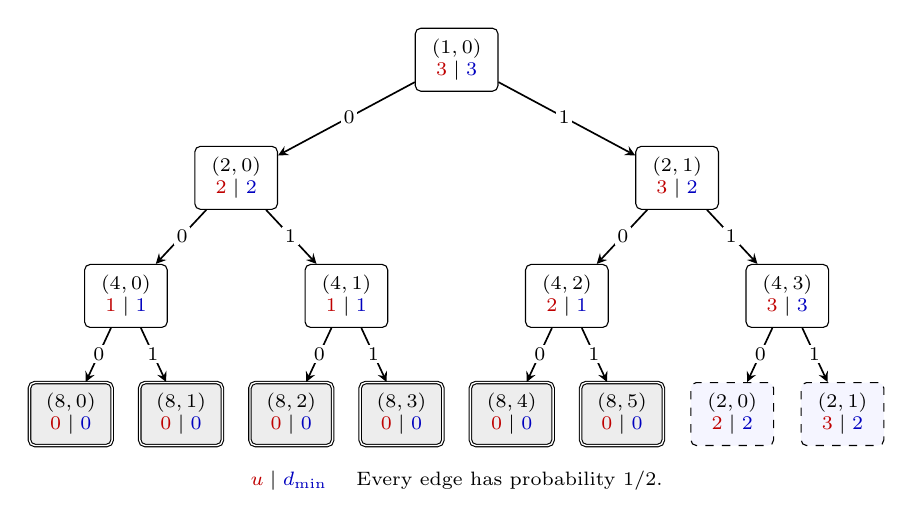
\begin{tikzpicture}[
   x=1.4cm,y=1cm,>=stealth,
   fdrstate/.style={draw,rounded corners=2pt,minimum width=10.5mm,
     minimum height=8mm,inner sep=2pt,align=center,font=\scriptsize},
   fdrterminal/.style={fdrstate,fill=black!7,double,double distance=0.5pt},
   fdrrecycled/.style={fdrstate,dashed,fill=blue!4},
   fdrbit/.style={font=\scriptsize,fill=white,inner sep=1pt},
   fdredge/.style={->,semithick}
 ]
 % Each node displays (v,c), then u | d_min.
 \node[fdrstate] (s10) at (3.5,4.5)
   {$(1,0)$\\$\textcolor{red!75!black}{3}\mid\textcolor{blue!75!black}{3}$};
 \node[fdrstate] (s20) at (1.5,3)
   {$(2,0)$\\$\textcolor{red!75!black}{2}\mid\textcolor{blue!75!black}{2}$};
 \node[fdrstate] (s21) at (5.5,3)
   {$(2,1)$\\$\textcolor{red!75!black}{3}\mid\textcolor{blue!75!black}{2}$};
 \node[fdrstate] (s40) at (0.5,1.5)
   {$(4,0)$\\$\textcolor{red!75!black}{1}\mid\textcolor{blue!75!black}{1}$};
 \node[fdrstate] (s41) at (2.5,1.5)
   {$(4,1)$\\$\textcolor{red!75!black}{1}\mid\textcolor{blue!75!black}{1}$};
 \node[fdrstate] (s42) at (4.5,1.5)
   {$(4,2)$\\$\textcolor{red!75!black}{2}\mid\textcolor{blue!75!black}{1}$};
 \node[fdrstate] (s43) at (6.5,1.5)
   {$(4,3)$\\$\textcolor{red!75!black}{3}\mid\textcolor{blue!75!black}{3}$};
 \foreach \j in {0,...,5} {
   \node[fdrterminal] (t\j) at (\j,0)
     {$(8,\j)$\\$\textcolor{red!75!black}{0}\mid\textcolor{blue!75!black}{0}$};
 }
 \node[fdrrecycled] (r20) at (6,0)
   {$(2,0)$\\$\textcolor{red!75!black}{2}\mid\textcolor{blue!75!black}{2}$};
 \node[fdrrecycled] (r21) at (7,0)
   {$(2,1)$\\$\textcolor{red!75!black}{3}\mid\textcolor{blue!75!black}{2}$};
 \foreach \from/\to/\bit in {
   s10/s20/0,s10/s21/1,
   s20/s40/0,s20/s41/1,s21/s42/0,s21/s43/1,
   s40/t0/0,s40/t1/1,s41/t2/0,s41/t3/1,
   s42/t4/0,s42/t5/1,s43/r20/0,s43/r21/1} {
   \draw[fdredge] (\from) -- node[fdrbit,pos=0.48] {$\bit$} (\to);
 }
 \node[font=\scriptsize,align=center] at (3.5,-0.85)
   {$\textcolor{red!75!black}{u}\mid\textcolor{blue!75!black}{d_{\min}}$
    \quad Every edge has probability $1/2$.};
 \end{tikzpicture}
 \caption{Three-iteration unfolding of FDR for $n=6$. Each node gives
 $(v,c)$ and, below it, the logarithmic variant $u$ (red, left) and the
 shortest distance $d_{\min}$ (blue, right). Edge labels are sampled bits.
 Double borders mark terminal states, where both functions are zero.
 Dashed leaves repeat earlier states after recycling; they are not
 terminal. Each edge includes all updates of one loop iteration.}
 \label{fig:fdr-iteration-variants}
\end{figure}

\begin{theorem}[AST of FDR]
\label{thm:fdr}
For every $n\in\mathbb{N}_{>0}$, FDR terminates almost surely.
\end{theorem}
\begin{proof}
Use the existing distributional invariant and define
\[
 v(\sigma)=
 \begin{cases}0&v\ge n,\\ n&v<n,\end{cases}
 \qquad
 u(\sigma)=
 \begin{cases}
 0&v\ge n,\\
 \left\lceil\log_2\!\left(\dfrac{n}{v-c}\right)\right\rceil&v<n.
 \end{cases}
\]
On enabled states, $1\leq v-c\leq n-1$, so $u$ is a positive integer.
The supermartingale obligation is immediate: $n$ is unchanged and every
successor is assigned either $n$ or $0$.
For progress, inspect the outcome generated by the left fair branch.
Its final difference is $2(v-c)$, irrespective of recycling. If the
successor remains enabled, then
\[
 u(\sigma')=
 \left\lceil\log_2\!\left(\frac{n}{2(v-c)}\right)\right\rceil
 =u(\sigma)-1.
\]
If it is terminal, $u(\sigma')=0<u(\sigma)$ instead. The left bit has
probability $1/2$, giving $\varepsilon=1/2$.

For every $r\geq0$, an enabled state in the sublevel set of the
supermartingale satisfies $n\leq r$. Hence, for $r\geq1$,
$u\leq\lceil\log_2 n\rceil\leq\lceil\log_2 r\rceil$ there.
For $r<1$ the sublevel set contains only terminal states, with $u=0$.
Thus $u$ is bounded on every sublevel set, also when $n$ ranges over all
positive integers. All obligations of \Cref{thm:program-rule} hold.
\end{proof}

\paragraph{Alternative variants.}
The exact shortest distance $d_{\min}$ is itself a valid variant for the
same supermartingale. From each enabled state, the first edge of a shortest
path leads to a successor with distance $d_{\min}-1$ and has probability
at least $1/2$. Moreover, \eqref{eq:fdr-shortest-distance-bound}, together
with the terminal value zero, gives $d_{\min}\leq u$, so the sublevel
bound just proved also applies to $d_{\min}$. We retain $u$ because it has
a simple explicit expression whose descent can be checked directly.

An even simpler algebraic alternative is the guarded affine function
\[
 \widetilde u(\sigma)=
 \begin{cases}
   n-v+c,&v<n,\\
   0,&v\geq n.
 \end{cases}
\]
On enabled states $1\leq\widetilde u\leq n-1$. A continuing zero-bit
successor has
$\widetilde u(\sigma')=\widetilde u(\sigma)-(v-c)
\leq\widetilde u(\sigma)-1$; a terminal successor has value zero.
Thus it also gives progress probability $1/2$, and
$\widetilde u\leq v(\sigma)$ gives sublevel boundedness.
Its active-state expression is affine in $(n,v,c)$, making it directly
accessible to an affine-template synthesis algorithm, whereas the
logarithmic expression requires a richer template language.
Indeed, the synthesis procedure in \Cref{sec:synthesis-examples} finds
this affine alternative for symbolic $n$. We keep the logarithmic
variant here to preserve its direct connection to the shortest-path
motivation and the pCFG comparison below.

\subsubsection{pCFG-Level Proof and Comparison.}
The same FDR argument can be stated using the pCFG rule of Majumdar and
Sathiyanarayana. Its graph separates the guard, assignments, fair choice,
conditional, and recycling updates. The loop head carries the support
predicate \eqref{eq:fdr-support}; intermediate locations carry its images
under the preceding assignments, including evenness of $v$ immediately
after doubling. Forgetting such information can make an intermediate
certificate undefined even when every reachable execution is well behaved.

For the explicit graph in \Cref{app:comparison}, set $V=n$ at every
nonterminal location and $V=0$ at the exit. A location-dependent natural
variant is obtained from the same logarithmic expression by multiplying
it by $7$, the maximum number of transitions in an iteration, and adding
control-location offsets. Its arguments account for partially executed
updates: immediately after doubling $v$, for example, the old difference
is $v/2-c$. Every deterministic edge strictly decreases this annotation;
the zero-bit edge decreases it with probability $1/2$. The appendix gives
the full invariant, annotation, and edge checks.

Both proofs establish the same AST result. At program level, the control
locations and offsets disappear: the proof uses one support predicate,
two state functions, and \eqref{eq:fdr-post}. It also retains the existing
distributional invariant for output correctness. This is a comparison of
proof representation, not an empirical claim about verification time.

\subsection{Fast Loaded Dice Roller: Rejection and Restart}
\label{sec:fldr}

The Fast Loaded Dice Roller (FLDR) samples outcome $i$ with probability
$a_i/m$, where $a_1,\ldots,a_n$ are positive integers and
$m=\sum_{i=1}^n a_i$~\cite{DBLP:conf/aistats/SaadFRM20}. Put
$k=\lceil\log_2m\rceil$ and add a rejecting outcome $n+1$ of weight
$2^k-m$. The binary expansions of these $n+1$ weights determine a finite
fair-bit decision tree: a set bit at position $k-c$ gives one leaf with
the corresponding label at depth $c$. Thus each label occurs at most
once per level and no internal node has two rejecting children.

We use a row-indexed presentation of this tree. Internal nodes come first
in each row, followed by leaves in decreasing label order. Write
$\phi_h(c)$ for the number of internal nodes in row $c$, and let
$H[d,c]$ be zero at an internal node and its output label at a leaf.
The two children of internal node $(c,d)$ have indices $2d$ and $2d+1$
in row $c+1$. This convention is also used by the concrete synthesis
example; it is an explicit tree presentation of FLDR, rather than the
array indexing of the original implementation.

Abstracting the terminating preprocessing, the sampling loop is:
\begin{lstlisting}[basicstyle=\ttfamily\small,mathescape=true,frame=single]
$c := 0;\ d := 0;$
while ($d < \phi_h(c)$) do
  $c := c+1;$
  $d := 2d$ [1/2] $d := 2d+1;$
  if ($H[d,c]=n+1$) then $c:=0;\ d:=0$ else skip
end
\end{lstlisting}
On termination it returns $H[d,c]$. If the root is already an accepting
leaf, the loop is skipped; this includes the single weight $a_1=2^k$,
in particular $m=1$. Otherwise the root is internal.

The support invariant says that $(c,d)$ is a valid, non-rejecting tree
node. In particular, its integer coordinates satisfy
\begin{equation}
 0\le c\le k,\qquad 0\le d<2n,
 \qquad d<\phi_h(c)\ \Longrightarrow\ c<k.
 \label{eq:fldr-support}
\end{equation}
The last implication excludes enabled states at maximal depth.
The row construction and these bounds are justified in
\Cref{app:calculations}. No probability-equality constraint from the
stronger distributional invariant is needed for AST.

\begin{theorem}[AST of FLDR]
\label{thm:fldr}
For every finite vector of positive integer weights, the FLDR sampling loop terminates almost surely.
\end{theorem}
\begin{proof}
Let $b$ be the loop guard. Define
\[
 v(\sigma)=\begin{cases}0&\sigma\not\models b,\\m&\sigma\models b,\end{cases}
 \qquad
 u(\sigma)=\begin{cases}0&\sigma\not\models b,\\k-c&\sigma\models b.\end{cases}
\]
Neither the weights nor $m$ are modified. Every post-state therefore has $v$ equal to $m$ if the loop remains enabled and $0$ otherwise, proving the supermartingale inequality.

Consider an enabled node. By \eqref{eq:fldr-support}, $c<k$, so
$u=k-c\geq1$. A non-rejecting child either continues at depth $c+1$,
decreasing $u$ by one, or accepts, decreasing $u$ to zero. At most one
child rejects, so such a decreasing outcome has probability at least
$1/2$. The other outcome may reset $(c,d)$ and increase $u$ back to $k$.

Finally, for $r\geq1$, every enabled state with $v\leq r$ satisfies
$m\leq r$, hence $u\leq k\leq\lceil\log_2r\rceil$.
For $0\leq r<1$ there are only terminal states and $u=0$.
This bound also covers a family of inputs with varying weights.
Thus \Cref{thm:program-rule} applies.
\end{proof}

This proof isolates the actual AST argument in three facts: $m$ is stable, tree height is logarithmically bounded by $m$, and at least one child avoids rejection. A direct pCFG treatment would additionally require values at the increment, choice, test, and reset locations, plus cases for both children. FLDR complements the FDR comparison by showing how the program-level rule accommodates rejection and restart through the post-distribution of one iteration.

\Cref{sec:synthesis-examples} reuses these structural facts as an input abstraction for certificate synthesis. With all scalar state variables and symbolic parameters available, the recorded shared-kernel run finds $v=[b]m$, $u=[b](m-c)$. For the concrete weights $(4,5)$, it also finds a common certificate depending on both depth and node index. Thus the resetting depth variant illustrates the flexibility of separate functions, without establishing that distinct functions are necessary for FLDR.

\paragraph{From AST to total correctness.}
The reused distributional invariants establish that the terminating FDR output is uniform and that FLDR returns $i$ with probability $a_i/m$~\cite{zilken2026verifyingsamplingalgorithmsdistributional}. \Cref{thm:fdr,thm:fldr} show AST, i.e. that the corresponding post-distributions have total mass one. Hence the partial-correctness distributions are proper output distributions, yielding total correctness for both algorithms.



\subsection{Han--Hoshi Sampling: Dyadic Refinement}
\label{sec:HanHoshi}

The fair-bit, finite-output instance of Han--Hoshi interval
sampling~\cite{HanHoshi1997} draws from a distribution with positive
integer weights $a_1,\ldots,a_n$ and total weight
$m=\sum_{i=1}^n a_i$.  Write $S_i=\sum_{j=1}^i a_j$, with $S_0=0$.
The algorithm repeatedly refines a dyadic interval until it lies entirely
inside one of the target intervals
\[
 I_i=\left[\frac{S_{i-1}}m,\frac{S_i}m\right),
 \qquad 1\le i\le n.
\]
Its sampling loop is:
\begin{lstlisting}[basicstyle=\ttfamily\small,mathescape=true,frame=single]
$v := 1;\ c := 0;\ r := 0;$
while ($r=0$) do
  $v := 2v;$
  $c := 2c$ [1/2] $c := 2c+1;$
  $r := \idx(c,v)$
end
\end{lstlisting}
Here
\[
 \idx(c,v)
 \coloneqq
 \begin{cases}
 i,
 & \text{if }S_{i-1}v\le cm\text{ and }(c+1)m\le S_iv
   \text{ for some }i\in\{1,\ldots,n\},\\
 0,&\text{if no such }i\text{ exists}.
 \end{cases}
\]
The pair $(c,v)$ represents the interval
\[
 J(c,v)=\left[\frac cv,\frac{c+1}v\right).
\]
At loop heads $v,c,r$ are integers, and the reachable states satisfy
\begin{equation}
 v>0,\qquad 0\le c<v,\qquad 0\le r\le n.
 \label{eq:han-hoshi-support}
\end{equation}
Moreover, after an iteration, $r=0$ exactly when the selected child
interval is not contained in a target interval.  As in the preceding case
studies, a stronger distributional invariant used for output correctness
may be retained; only the support information above is needed for AST.

Let $B_{\mathrm{HH}}$ denote the loop body.  For $b\in\{0,1\}$, set
\[
 c_b=2c+b,\qquad v'=2v,\qquad r_b=\idx(c_b,v').
\]
For a Dirac input $\dirac{\sigma}$,
\begin{equation}
 \post{B_{\mathrm{HH}}}(\dirac{\sigma})
 =\tfrac12\dirac{\sigma[v/v',c/c_0,r/r_0]}
 +\tfrac12\dirac{\sigma[v/v',c/c_1,r/r_1]}.
 \label{eq:han-hoshi-post}
\end{equation}
Thus one complete program-level step is precisely a fair choice between
the left and right halves of $J(c,v)$.

\begin{theorem}[AST of Han--Hoshi]
 \label{thm:han-hoshi}
For every finite vector of positive integer weights, the Han--Hoshi
sampling loop terminates almost surely.
\end{theorem}
\begin{proof}
For a reachable state $\sigma$, let
\[
 N(\sigma)
 =\left|\left\{i\in\{1,\ldots,n-1\}\,\middle|\,
 \frac cv<\frac{S_i}{m}<\frac{c+1}{v}\right\}\right|
\]
be the number of internal target boundaries lying strictly inside
$J(c,v)$.  Define the two certificates
\[
 \mathsf V(\sigma)=\mathsf U(\sigma)=
 \begin{cases}
 0,&r\ne0,\\
 \max\{1,N(\sigma)\},&r=0.
 \end{cases}
\]
They vanish exactly on terminal states, and $\mathsf U$ is
natural-valued.

Consider an enabled state and write $q=N(\sigma)$.  Splitting $J(c,v)$
into its two children cannot create an internal target boundary.  Every
boundary counted in a child is counted in the parent, while a boundary at
the common endpoint of the children is counted in neither.  If $N_b$
denotes the number of boundaries strictly inside child $b$, then
\begin{equation}
 N_0+N_1\le q.
 \label{eq:han-hoshi-boundary-split}
\end{equation}
Since the target intervals partition $[0,1)$ and every child lies in
$[0,1)$, a child is contained in one target interval exactly when its
interior contains no target boundary. This also handles boundaries at
endpoints, which are not counted. Thus a child remains enabled exactly
when it contains an internal boundary in its interior; hence its post-state certificate is $N_b$ if $N_b>0$ and
zero otherwise.  Using \eqref{eq:han-hoshi-post} and
\eqref{eq:han-hoshi-boundary-split}, for $q>0$ we obtain
\[
 \mathbb E_\sigma[\mathsf V']
 =\tfrac12(N_0+N_1)
 \le\tfrac q2
 \le \mathsf V(\sigma).
\]
If $q=0$, both children are terminal and the expectation is zero.  This
proves the supermartingale obligation of \Cref{thm:program-rule}.

For the decrease obligation, if $q>0$, at least one of $N_0,N_1$ is
strictly smaller than $q$: otherwise their sum would be at least $2q$,
contradicting \eqref{eq:han-hoshi-boundary-split}.  The corresponding
post-state therefore has strictly smaller $\mathsf U$.  It is selected
with probability $1/2$, so the decrease condition holds with
$\varepsilon=1/2$.  If $q=0$, both children terminate and decrease
$\mathsf U$ from $1$ to $0$, so the same bound applies.

Finally, $\mathsf U=\mathsf V$ on every reachable state.  Consequently,
on each sublevel set $\mathsf V_{\le R}$ we have
$\mathsf U\le R$.  All obligations of \Cref{thm:program-rule} hold, and
the loop is AST.
\end{proof}

\paragraph{Illustrating the two certificate roles.}
For weights $(a_1,a_2)=(1,2)$, the only internal target boundary is
$1/3$.  Hence every enabled state has $\mathsf V=\mathsf U=1$.
\Cref{fig:han-hoshi-certificates} shows the first two refinements.
Exactly one child still straddles $1/3$ and retains value $1$; the
other is contained in a target interval and has value $0$.
Thus, at either enabled state shown,
\[
 \underbrace{\mathbb E_\sigma[\mathsf V']
 =\tfrac12\cdot1+\tfrac12\cdot0
 =\tfrac12\le\mathsf V(\sigma)}_{\text{supermartingale obligation}},
 \qquad
 \underbrace{\Pr\nolimits_\sigma\!\left(\mathsf U'<\mathsf U(\sigma)\right)
 =\tfrac12}_{\text{variant decrease}}.
\]
The continuing branch need not decrease the variant, and the decreasing
bit changes between the two refinements.  The same function therefore
meets two different obligations: non-increase in expectation and strict
decrease with uniformly positive probability.  Sublevel-set boundedness
is immediate from $\mathsf U=\mathsf V$.

\begin{figure}[tbp]
 \centering
 % Uses only TikZ and xcolor, already loaded in packages.tex.
 % Horizontal positions are fractions of the unit interval.
 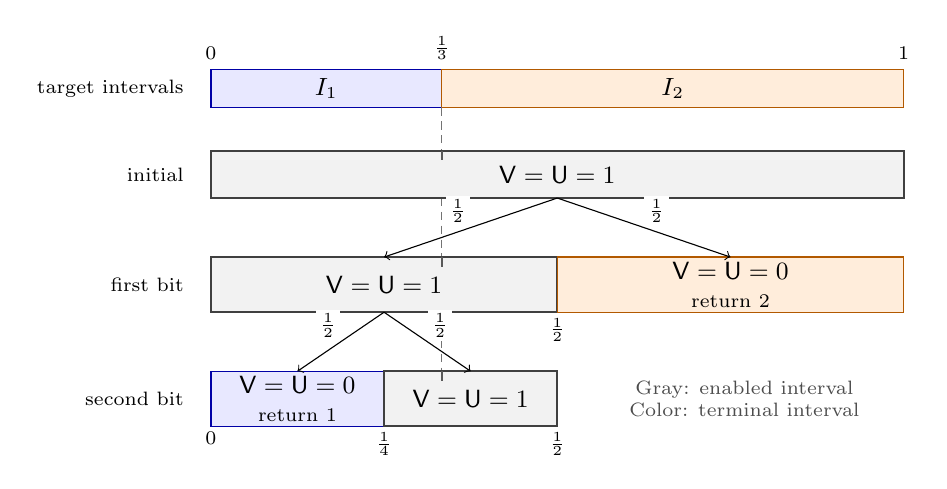
\begin{tikzpicture}[
   x=8.8cm,y=1cm,
   every node/.style={font=\small},
   active/.style={draw=black!75,fill=black!5,line width=.7pt},
   first/.style={draw=blue!65!black,fill=blue!9,line width=.5pt},
   second/.style={draw=orange!70!black,fill=orange!14,line width=.5pt},
   bit/.style={font=\scriptsize,fill=white,inner sep=1.5pt},
   rowlabel/.style={anchor=east,font=\scriptsize,align=right}
 ]
  % The target distribution, with its unique internal boundary.
  \path[first]  (0,0) rectangle (1/3,.48);
  \path[second] (1/3,0) rectangle (1,.48);
  \node at (1/6,.24) {$I_1$};
  \node at (2/3,.24) {$I_2$};
  \node[rowlabel] at (-.025,.24) {target\ intervals};
  \node[above,font=\scriptsize] at (0,.48) {$0$};
  \node[above,font=\scriptsize] at (1/3,.48) {$\tfrac13$};
  \node[above,font=\scriptsize] at (1,.48) {$1$};

  % Put the guide behind the arrows and their probability labels.
  \draw[densely dashed,black!55] (1/3,0) -- (1/3,-.55);
  \draw[densely dashed,black!55] (1/3,-1.15) -- (1/3,-1.90);
  \draw[densely dashed,black!55] (1/3,-2.60) -- (1/3,-3.35);

  % The initial interval J(0,1).
  \path[active] (0,-1.15) rectangle (1,-.55);
  \node at (.5,-.85) {$\mathsf V=\mathsf U=1$};
  \node[rowlabel] at (-.025,-.85) {initial};

  % First fair bit: left child continues, right child returns outcome 2.
  \path[active] (0,-2.60) rectangle (.5,-1.90);
  \path[second] (.5,-2.60) rectangle (1,-1.90);
  \node at (.25,-2.25) {$\mathsf V=\mathsf U=1$};
  \node[align=center] at (.75,-2.25)
    {$\mathsf V=\mathsf U=0$\\[-1pt]\scriptsize return $2$};
  \node[rowlabel] at (-.025,-2.25) {first\ bit};
  \draw[->] (.5,-1.15) -- node[bit,above left] {$\tfrac12$} (.25,-1.90);
  \draw[->] (.5,-1.15) -- node[bit,above right] {$\tfrac12$} (.75,-1.90);
  \node[below,font=\scriptsize,inner sep=2pt] at (.5,-2.60) {$\tfrac12$};

  % Refine only the still-enabled left child.
  \path[first]  (0,-4.05) rectangle (.25,-3.35);
  \path[active] (.25,-4.05) rectangle (.5,-3.35);
  \node[align=center] at (.125,-3.70)
    {$\mathsf V=\mathsf U=0$\\[-1pt]\scriptsize return $1$};
  \node at (.375,-3.70) {$\mathsf V=\mathsf U=1$};
  \node[rowlabel] at (-.025,-3.70) {second\ bit};
  \draw[->] (.25,-2.60) -- node[bit,above left] {$\tfrac12$} (.125,-3.35);
  \draw[->] (.25,-2.60) -- node[bit,above right] {$\tfrac12$} (.375,-3.35);
  \node[below,font=\scriptsize,inner sep=2pt] at (0,-4.05) {$0$};
  \node[below,font=\scriptsize,inner sep=2pt] at (.25,-4.05) {$\tfrac14$};
  \node[below,font=\scriptsize,inner sep=2pt] at (.5,-4.05) {$\tfrac12$};

  % Short boundary ticks at the top of each enabled interval.
  \draw[black!65,line width=.6pt] (1/3,-.55) -- (1/3,-.67);
  \draw[black!65,line width=.6pt] (1/3,-1.90) -- (1/3,-2.02);
  \draw[black!65,line width=.6pt] (1/3,-3.35) -- (1/3,-3.47);
  \node[align=center,font=\scriptsize,text=black!70] at (.77,-3.70)
    {Gray: enabled interval\\Color: terminal interval};
 \end{tikzpicture}
 \caption{Han--Hoshi for weights $(1,2)$.  Bars represent half-open
 intervals at their actual horizontal positions; the dashed guide marks
 the target boundary $1/3$.  A gray interval straddles this boundary and
 has $\mathsf V=\mathsf U=1$; a colored interval is contained in $I_1$ or
 $I_2$ and has value $0$.  Arrows show conditional probabilities for one
 complete loop iteration.  Only the enabled child is refined further.}
 \label{fig:han-hoshi-certificates}
\end{figure}


The proof replaces the explicit depth-$t$ tail calculation by one
iteration-level fact: bisecting an interval distributes its internal
target boundaries over the two children, and at least one child contains
strictly fewer.  The number of such boundaries serves simultaneously as
the supermartingale and the natural-valued variant (with the value $1$
for the enabled boundary-free initial case).  Hence Han--Hoshi supplies a further application of the
program-level rule of \Cref{thm:program-rule}, with a certificate based on
interval refinement rather than the progress-and-restart structure of
FDR and FLDR.

\section{Template-Based Certificate Synthesis}
\label{sec:certificate-synthesis}

The iteration-level obligations of \Cref{thm:program-rule} admit a direct
constraint-based instantiation. We implement a shared counterexample-guided
inductive synthesis (CEGIS) kernel for the random walk, FDR, and FLDR.
It searches for two independent certificates using guarded affine templates,
optionally refined by a supplied finite partition. The contribution is a
reproducible feasibility demonstration for these obligations, rather than a
new general-purpose synthesis method.

\subsection{Templates and Verification Conditions}
\label{sec:synthesis-constraints}

The input comprises integer state variables, immutable integer parameters,
a guard $b$, an initial-state description, a supplied inductive predicate
$S$, and a manually encoded complete body step. There is no program parser
or invariant synthesis. Every declared integer component is included in the
automatic feature vector $\mathbf{x}=(x_1,\ldots,x_d)$; Boolean flags may
occur in the guard but are not numerical features. Fixed numerical inputs
are substituted into the semantics. Symbolic parameters remain features.
The two templates are
\[
 V_{\mathbf a}(\sigma)=[b](\sigma)
   \Bigl(a_0+\sum_{i=1}^d a_i x_i(\sigma)\Bigr),\qquad
 U_{\mathbf u}(\sigma)=[b](\sigma)
   \Bigl(u_0+\sum_{i=1}^d u_i x_i(\sigma)\Bigr),
\]
with independent integer coefficients. The basis construction is automatic;
the supplied state representation and affine hypothesis class are not.

The paper inputs have two equiprobable complete outcomes $T_0,T_1$.
For an abstract input, an additional relation $A(\sigma,\xi)$ describes
admissible outcome pairs $T_0(\sigma,\xi),T_1(\sigma,\xi)$ using auxiliary
descriptors $\xi$, which are excluded from the feature vector. Every enabled
state must admit a pair, and every concrete outcome pair must be represented.
The latter is a separate semantic justification of the abstraction.
Suppressing $\xi$, we require on $S\land b$, for every admissible pair,
\begin{align}
 V(\sigma)&\geq1,& U(\sigma)&\geq1,
 \label{eq:syn-positive}\\
 V(T_0(\sigma))+V(T_1(\sigma))&\leq2V(\sigma),
 \label{eq:syn-supermartingale}\\
 U(T_0(\sigma))\leq U(\sigma)-1
 &\quad\lor\quad U(T_1(\sigma))\leq U(\sigma)-1,
 \label{eq:syn-progress}\\
 U(\sigma)&\leq V(\sigma).
 \label{eq:syn-domination}
\end{align}
Domination is sufficient for sublevel boundedness, but stronger than the
premise of \Cref{thm:program-rule}; integer coefficients and $V\geq1$
also restrict the search.

\begin{proposition}[Soundness of the synthesis constraints]
\label{prop:synthesis-soundness}
Suppose $S$ contains the initial states and is preserved by all represented
outcomes. If an abstraction is used, suppose it represents every concrete
outcome pair. Every instantiation satisfying
\eqref{eq:syn-positive}--\eqref{eq:syn-domination} supplies an AST
certificate with $\varepsilon=1/2$.
\end{proposition}
\begin{proof}
Both templates vanish on terminal states. On active states $V$ is positive
and $U$ is a positive integer. The expectation inequality applies to each
concrete body distribution, and at least one fair-bit outcome decreases
$U$ by one. On $V\leq r$, domination bounds $U$ by $\lfloor r\rfloor$.
Subdistributions supported in $S$ form a distributional invariant. These are
precisely the required premises of \Cref{thm:program-rule}.
\end{proof}

\subsection{Finite Search and Supplied Partitions}
\label{sec:synthesis-cegis}

For a fixed bound $B$, every coefficient ranges over $\{-B,\ldots,B\}$.
An SMT query chooses an enabled initial sample automatically, including
admissible descriptors when needed. The learner selects both coefficient
vectors simultaneously, satisfying all obligations on accumulated samples
and minimizing the sum of absolute coefficients. This objective favors
small expressions; it has no soundness role, and solver ties remain open.
The verifier fixes the coefficients and asks for any state in $S\land b$
(and admissible descriptor) violating an obligation. A satisfying assignment
is added to the samples. An unsatisfiable query verifies the candidate over
the \emph{entire} invariant domain, including unbounded integer parameters.
It is not a bounded-state test.

With a sample fixed, learner constraints are linear in the unknown
coefficients; with coefficients fixed, verifier constraints are linear in
the unknown state and descriptor variables. The supplied examples use only
Boolean combinations of linear arithmetic and piecewise affine updates.
The implementation checks initialization and preservation of $S$ separately.
For abstract inputs it also checks
$S\land b\Rightarrow\exists\xi\,A(\sigma,\xi)$; this coverage query can
contain quantification. Nonempty coverage prevents vacuous verification but
does not prove correspondence with a concrete program.

Every counterexample excludes at least the current candidate and no valid
candidate. Consequently, with exact terminating solvers and no resource
limits, the procedure terminates and is complete for a \emph{fixed finite}
template and these sufficient constraints. The implementation tries
$B=1,2,4,8,16$, retaining samples between bounds. Learner unsatisfiability
excludes only the current bounded template. Unknown results, timeouts, and
the 500-candidate limit are inconclusive. Neither the finite schedule nor
relative completeness of the proof rule establishes synthesis completeness
for AST programs.

\paragraph{Fixed piecewise affine templates.}
\label{sec:synthesis-piecewise}
The same kernel accepts a supplied partition $P_1,\ldots,P_q$ of active
invariant states, checks coverage and pairwise disjointness, and assigns an
independent full affine coefficient block to each region and each function:
\[
 V(\sigma)=[b](\sigma)\sum_{j=1}^{q}[P_j](\sigma)
 \left(a_{j,0}+\sum_{i=1}^{d}a_{j,i}x_i(\sigma)\right).
\]
The $U$-template is analogous. Predicates may use declared state components,
but not auxiliary transition descriptors or undeclared symbols. Region
selection is reevaluated at every successor, including cross-region
transitions. The constraints and soundness argument are unchanged.
A threshold split $e<r$ versus $e\geq r$ supplies both expressions;
$r$ may be a numeral or a linear expression in symbolic parameters.
Thresholds and partitions are not synthesized. Extra regions enlarge the
finite search space; they are not assumed to improve performance.

\subsection{Reproduced Results and Their Scope}
\label{sec:synthesis-examples}

\Cref{tab:synthesis-results} reports the delivered artifact run with
Z3~4.15.4 and ten seconds per solver call. The same engine, coefficient
schedule, and objective are used throughout. All final obligations are
rechecked separately. Recorded coefficient vectors, samples, counterexamples,
bound attempts, and measured wall times accompany the code; candidate counts
can vary with solver tie-breaking. These experiments are feasibility checks,
not a performance comparison with other tools.

\begin{table}[t]
\centering\small
\setlength{\tabcolsep}{4pt}
\begin{tabular}{@{}llllr@{}}
\toprule
Input & $V$ & $U$ & $B$ & Candidates\\
\midrule
Random walk & $x$ & $x$ & 1 & 2\\
FDR, symbolic $n$ & $n$ & $n-v+c$ & 1 & 3\\
FLDR, weights $(4,5)$ & $c-2d+2$ & $c-2d+2$ & 2 & 4\\
FLDR, abstract family & $m$ & $m-c$ & 1 & 4\\
Two-sided walk, supplied split & $|x|$ & $|x|$ & 1 & 4\\
\bottomrule
\end{tabular}
\caption{Synthesized expressions on active states, with terminal values zero.
$B$ is the successful bound; candidate counts include earlier bounds.
The abstract FLDR row is conditional on the structural contract below.}
\label{tab:synthesis-results}
\end{table}

\paragraph{Unbounded symmetric random walk.}
For \Cref{sec:walk}, $S\equiv x\geq0$ yields features $(x,1)$ and the
verified result $V=U=x$. The expectation is unchanged, while the left outcome
decreases $U$ by one. This establishes AST despite infinite expected runtime:
for $0<x<N$, the expected time $x(N-x)$ to hit $\{0,N\}$ lower-bounds
the time to hit $0$, and diverges with $N$.
A uniform negative expected drift is unnecessary.

\paragraph{FDR with a symbolic range.}
For the loop of \Cref{sec:fdr}, the supplied invariant is
$S\equiv n\geq1\land1\leq v<2n\land0\leq c<v\land c<n$, and the
complete bit-$\beta$ update is
\[
 T_\beta(n,v,c)=
 \begin{cases}
 (n,2v-n,2c+\beta-n),&2c+\beta\geq n,\\
 (n,2v,2c+\beta),&2c+\beta<n.
 \end{cases}
\]
The full basis $(n,v,c,1)$ yields $V=n$, $U=n-v+c$ on $v<n$,
uniformly for symbolic $n$. Put $\Delta=v-c$. Enabled states satisfy
$1\leq\Delta\leq n-1$ and $U=n-\Delta$. On bit zero a continuing
successor has $\Delta'=2\Delta$, giving $U'\leq U-1$; acceptance
sets $U'=0$. Since $n$ is unchanged, $V'$ is $n$ or zero, and $U\leq V$.
Thus an affine variant suffices in place of the manual logarithmic one.
FDR remains a baseline for the separation of certificate roles: on bit one,
$\Delta'=2\Delta-1\geq\Delta$ when continuing, so in fact
$\mathbb E[U']\leq U-1/2$. This additional inequality is independently
SMT-verified; $U$ itself is a ranking supermartingale here.

\paragraph{FLDR with fixed weights.}
For $(4,5)$, preprocessing gives $m=9$, $k=4$, and rejection weight $7$.
The artifact constructs the exact finite tree from binary weight columns,
placing internal nodes before leaves and leaf labels in descending order,
as in \Cref{sec:fldr}. The supplied invariant is its set of loop-head nodes;
the feature basis is $(c,d,1)$. After excluding $B=1$, the engine finds
$V=U=c-2d+2$ at $B=2$. \Cref{fig:fldr-synthesis-tree} displays the
five active nodes, acceptances, and resets. An independent rational-arithmetic
audit checks all nodes and edges (\Cref{app:artifact}). At the root the
expectation is unchanged, so this shared certificate has no uniform
negative drift.
\begin{figure}[tbp]
 \centering
 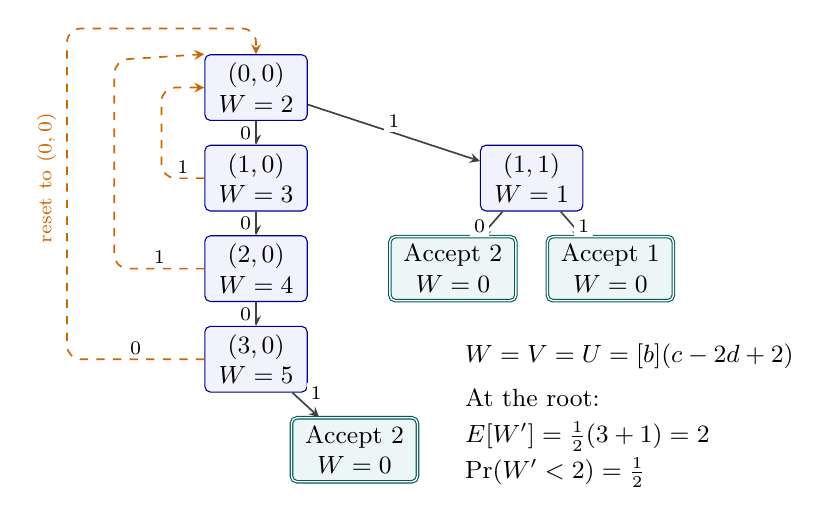
\begin{tikzpicture}[
   x=1cm,y=1cm,>=stealth,
   fldrnode/.style={draw=blue!55!black,fill=blue!5,rounded corners=2pt,
     minimum width=13mm,minimum height=8mm,inner sep=3pt,
     align=center,font=\small},
   fldraccept/.style={draw=teal!70!black,fill=teal!7,
     double,double distance=.5pt,rounded corners=2pt,
     minimum width=16mm,inner sep=3pt,align=center,font=\small},
   fldredge/.style={->,semithick,draw=black!75},
   fldrreset/.style={->,semithick,dashed,draw=orange!80!black,
     rounded corners=5pt},
   fldrbit/.style={font=\scriptsize,fill=white,inner sep=1.5pt}
 ]
 \node[fldrnode] (root) at (0,0) {$(0,0)$\\$W=2$};
 \node[fldrnode] (s10) at (0,-1.15) {$(1,0)$\\$W=3$};
 \node[fldrnode] (s11) at (3.5,-1.15) {$(1,1)$\\$W=1$};
 \node[fldrnode] (s20) at (0,-2.30) {$(2,0)$\\$W=4$};
 \node[fldrnode] (s30) at (0,-3.45) {$(3,0)$\\$W=5$};
 \node[fldraccept] (a22) at (2.5,-2.30)
   {Accept $2$\\$W=0$};
 \node[fldraccept] (a23) at (4.5,-2.30)
   {Accept $1$\\$W=0$};
 \node[fldraccept] (a41) at (1.25,-4.60)
   {Accept $2$\\$W=0$};

 % Each arrow includes every update of one loop-body execution.
 \draw[fldredge] (root) -- node[fldrbit,left] {$0$} (s10);
 \draw[fldredge] (root) -- node[fldrbit,above] {$1$} (s11);
 \draw[fldredge] (s10) -- node[fldrbit,left] {$0$} (s20);
 \draw[fldredge] (s11) -- node[fldrbit,pos=.58,left] {$0$} (a22);
 \draw[fldredge] (s11) -- node[fldrbit,pos=.58,right] {$1$} (a23);
 \draw[fldredge] (s20) -- node[fldrbit,left] {$0$} (s30);
 \draw[fldredge] (s30) -- node[fldrbit,above right] {$1$} (a41);

 % Reset events are contracted into their bit-labelled body transitions;
 % raw rejecting leaves are not loop-head states and get no certificate value.
 \draw[fldrreset] (s10.west) -- node[fldrbit,above] {$1$}
   (-1.20,-1.15) -- (-1.20,0) -- (root.west);
 \draw[fldrreset] (s20.west) -- node[fldrbit,above] {$1$}
   (-1.80,-2.30) -- (-1.80,.35) -- (root.north west);
 \draw[fldrreset] (s30.west) -- node[fldrbit,above] {$0$}
   (-2.40,-3.45) -- (-2.40,.75) -- (0,.75) -- (root.north);
 \node[font=\scriptsize,text=orange!80!black,rotate=90]
   at (-2.66,-1.15) {reset to $(0,0)$};

 \node[align=left,font=\small,anchor=north west,inner sep=0pt]
   at (2.65,-3.25)
   {$W=V=U=[b](c-2d+2)$\\[5pt]
    At the root:\\[2pt]
    $\mathbb E[W']=\tfrac12(3+1)=2$\\[2pt]
    $\Pr(W'<2)=\tfrac12$};
 \end{tikzpicture}
 \caption{A decision tree for FLDR with weights $(4,5)$ and rejection
 weight $7$. Active nodes show $(c,d)$ and the shared certificate value
 $W$; double-bordered leaves accept the indicated outcome and have value
 zero. Every edge represents one complete iteration with probability
 $1/2$; its label is the sampled bit. Dashed edges include rejection and
 reset, returning to the root with $W=2$. The root calculation illustrates
 progress despite zero expected decrease.}
 \label{fig:fldr-synthesis-tree}
\end{figure}

\paragraph{FLDR under a symbolic structural contract.}
For arbitrary trees, the input retains all integer components $(m,k,n,c,d)$
and uses a Boolean activity flag for the guard. Its support requires
$m\geq1$, $0\leq k\leq m$, $1\leq n\leq m$, $0\leq c\leq k$,
$d\geq0$, and $\mathit{active}\Rightarrow c<k$. Each bit outcome is
classified as continuation, rejection, or acceptance. Continuation advances
to $(c+1,2d+\beta)$ and requires $c+1<k$; rejection resets to $(0,0)$;
acceptance advances to the child and disables the guard. Parameters are
unchanged, and both outcomes may not reject simultaneously.

Tree height at most $k$ and at most one rejecting leaf per level justify
this contract (\Cref{sec:fldr}). The certificate solver does not derive these
facts from preprocessing. The domain overapproximates
$k=\lceil\log_2m\rceil$ and avoids logarithmic arithmetic.
The full basis $(m,k,n,c,d,1)$ yields $V=m$, $U=m-c$ on active states;
all irrelevant coefficients become zero without a prescribed feature subset.
Every successor has $V'$ equal to $m$ or zero, a nonrejecting outcome
decreases $U$ by at least one, and $1\leq U=m-c\leq m=V$.
The alternative pair $V=k$, $U=k-c$ is also independently verified,
but is not the candidate selected in the recorded affine run.

The depth variant can grow in expectation: at $(c,d)=(2,0)$ in the fixed
tree, $U=2$ but $\mathbb E[U']=5/2$. In the restricted basis $(k,c,1)$,
a shared function at $k=4$ has the form $W(c)=A+Dc$. Progress at the root
forces $D<0$, while its expected change at $(2,0)$ is then $-D/2>0$.
However, the synthesized $c-2d+2$ removes this obstruction. This separation
concerns a specified template class, not an intrinsic need for distinct
functions in FLDR.

\paragraph{What the supplied partition adds.}
For the symmetric walk on all of $\mathbb Z$, take guard $x\neq0$ and
support $\mathit{true}$. An affine variant $ax+b$ positive on both unbounded
tails must have $a=0$, and a constant cannot decrease at $x=2$. Hence no
single-affine pair satisfies the constraints, regardless of its coefficient
bound. With the supplied split $x<0$ versus $x\geq0$, the same kernel
synthesizes and universally verifies $V=U=|x|$. This is an expressiveness
check for a single template over the full invariant; two manual proofs on
sign-invariant domains would also suffice. Optional sampler partitions and
checks of cross-region transitions are documented in \Cref{app:artifact}.

The experiments establish neither unrestricted synthesis completeness nor
superiority to existing synthesis tools. Supplied invariants and semantics,
the FLDR abstraction, fixed partitions, and $U\leq V$ remain substantive
restrictions. Automatic extraction of semantics and partition selection are
outside the implemented scope.

\section{Related Work}
\label{sec:relwork}

\paragraph{AST proof rules.}
Bounded variants establish AST through a uniformly positive probability
of descent in a bounded natural-valued range~\cite{DBLP:series/mcs/McIverM05}.
McIver et al.~\cite{10.1145/3158121} give a source-level rule, including
demonic choice, in which a single real-valued function satisfies both
supermartingale and probabilistic progress obligations. Majumdar and
Sathiyanarayana~\cite{DBLP:journals/pacmpl/MajumdarS25} separate these roles
at pCFG level and prove relative completeness in arithmetic, also
establishing completeness of the earlier single-function rule.
Our contribution concerns the representation of certificates and their
transfer to whole iterations, rather than greater semantic proving power.
Separating the roles allows a resetting variant without requiring that
particular variant to be a supermartingale; it does not show that every
single-function certificate must fail.

The program-level transfer originates in Seidel's master's
thesis~\cite{seidel2026thesis}, whose Chapter~6 presents the two-certificate
rule and translations between program and pCFG certificates. The present
paper develops that foundation with explicit normalization and boundedness
arguments, sampler case studies, and a reproducible synthesis prototype.

\paragraph{Distribution transformers and program logics.}
Kozen's semantics~\cite{DBLP:conf/focs/Kozen79,DBLP:conf/stoc/Kozen83}
provides the denotational foundation for our post-distribution
transformers. Expectation-transformer reasoning~\cite{DBLP:series/mcs/McIverM05}
and distributional program logics, including den Hartog and de
Vink~\cite{DBLP:journals/ijfcs/HartogV02} and
Ellora~\cite{DBLP:conf/esop/BartheEGGHS18}, support broader probabilistic
correctness properties. Our AST rule complements such reasoning:
distributional invariants can carry output information, while termination
uses their support and two state functions. Thus, the rule does not
replace distributional output-correctness arguments.

\paragraph{Certificate and invariant synthesis.}
Constraint-based synthesis already supports martingales and ranking
supermartingales~\cite{ChakarovSankaranarayanan2013}. Batz et
al.~\cite{BatzEtAl2023} use counterexample-guided synthesis of piecewise
linear quantitative invariants at source level, including for
infinite-state programs. Their objectives include expected-outcome bounds
and finite expected runtime. We instantiate this search pattern with two AST certificates and the
sufficient coupling $U\leq V$. The random
walk illustrates qualitative termination with infinite expected runtime.
Neither CEGIS nor affine or piecewise affine templates are new here.
The contribution is their explicit instantiation for these two
iteration-level certificate roles. Invariants, transition summaries,
feature bases, and partitions remain supplied inputs; bounded search is
incomplete even though successful candidates are checked universally
over the encoded states.

Haase et al.~\cite{haase2026generatingfunctionsmeetoccupation} synthesize
occupation invariants represented by generating functions. Such
invariants describe expected visit counts and support exact inference,
with positive AST obtainable under suitable finiteness conditions.
Their unknowns and verification conditions therefore differ from our
state-function certificates for qualitative AST. Template instantiation
is common to both approaches, but their results are not interchangeable.

\paragraph{Exact samplers and their verification.}
The algorithms studied here are established constructions:
Lumbroso's FDR~\cite{DBLP:journals/corr/abs-1304-1916}, Saad et al.'s
FLDR~\cite{DBLP:conf/aistats/SaadFRM20}, and Han and Hoshi's interval
algorithm~\cite{HanHoshi1997}. Zilken et
al.~\cite{zilken2026verifyingsamplingalgorithmsdistributional} already
verify partial and total correctness of FDR and FLDR using
distributional invariants. We reuse those invariants and revisit AST
through the two-certificate rule. Han--Hoshi supplies a different
termination argument, rather than a new output-correctness proof.
Bagnall et al.'s Zar compiler~\cite{DBLP:journals/pacmpl/Bagnall0023}
verifies compilation of probabilistic programs into random-bit samplers
in Coq. Our handwritten proofs and solver-backed prototype do not
provide that level of mechanization.

\paragraph{Nondeterminism.}
Both AST rules above support demonic nondeterminism. Our current
transformer assigns one post-distribution to each input. Extending the
rule to universal scheduler quantification requires corresponding
semantic and progress obligations. Programmatic strategy
synthesis~\cite{DBLP:journals/pacmpl/BatzBKW24} instead resolves
nondeterminism to obtain a selected program; it addresses a different
quantification over choices.

\section{Conclusion}
\label{sec:conclusion}

We presented a program-level formulation of the two-certificate AST rule
and proved it sound and relatively complete for fixed-probability loops
with loop-free bodies. The certificate translations expose the work saved
at the source interface: users reason about the body's post-distribution
and supply two state functions, while the metatheory accounts for internal
control locations. Distributional partial-correctness invariants can be
retained, although termination uses only their supports.

The sampler proofs illustrate different progress mechanisms: recycling in
FDR, depth advancement with resets in FLDR, and boundary elimination in
Han--Hoshi. They do not establish that distinct certificates are always
necessary. In particular, concrete FLDR admits a shared certificate when
node indices are available, despite the failure of a shared depth-only
one. The random walk separates qualitative AST from finite expected runtime.

One bounded CEGIS kernel synthesizes guarded affine certificates and
piecewise affine certificates for fixed partitions. Its final
queries verify the constraints over the full supplied invariant domains.
This provides reproducible evidence for the certificate interface, not an
end-to-end verifier: invariants, iteration semantics, partitions, and the
FLDR abstraction are supplied, and $U\leq V$ restricts sublevel boundedness.
The rule's relative completeness does not transfer to this search.

Nested loops require AST summaries for inner executions and a new
compositional theorem: unbounded inner executions invalidate our bounded-path
translation argument.

For nondeterministic programs, \emph{demonic} semantics requires AST under
every scheduler resolving the choices. Extending our rule would therefore
require invariant preservation and the supermartingale condition for all
admissible body distributions, together with a uniform progress guarantee
for the variant. Checking only one selected distribution would cover only
the corresponding behavior. Establishing soundness of this extension remains
future work.

Automatic input generation, richer templates, and broader comparative
evaluation remain separate tasks.


\ifappendixversion
\appendix
\section{Translation and AST Preservation}
\label{app:translation}

\paragraph{Well-defined loop semantics.}
The transformer domain $\mathcal{H}$ from \Cref{sec:prelims} has pointwise suprema of increasing $\omega$-chains: these preserve $\omega$-continuity and the mass bound by monotone convergence. Its least element is $\bot=\lambda\eta.0$. By structural induction, the body transformer $\post{B}$ is $\omega$-continuous and does not increase mass. For $f\in\mathcal{H}$ and $\eta\in\subdists$,
\[
 \weight{\Phi_{b,B}(f)(\eta)}
 =\weight{[\neg b]\eta}
   +\weight{f\bigl(\post{B}([b]\eta)\bigr)}
 \leq\weight{[\neg b]\eta}+\weight{[b]\eta}
 =\weight{\eta}.
\]
Composition and addition preserve $\omega$-continuity here, so $\Phi_{b,B}(f)\in\mathcal{H}$. Moreover, for every increasing chain $(f_n)_n$ in $\mathcal{H}$, pointwise evaluation gives $\Phi_{b,B}(\sup_n f_n)=\sup_n\Phi_{b,B}(f_n)$. Kleene's theorem therefore yields \Cref{eq:while-transformer-fixpoint}. Structural induction also establishes linearity on sums that are subdistributions: in the loop case, every approximant is linear, and its pointwise supremum remains linear. The countable-sum property follows from $\omega$-continuity.

\paragraph{Operational correspondence.}
The translation $\mathcal{T}$ assigns distinct entry and exit locations to each command, with fresh internal locations for its subcommands. Skip is a single identity edge. Assignments are single update edges. A conditional entry has guarded edges to the two branch entries; a probabilistic-choice entry instead has edges of probabilities $p$ and $1-p$. In either case the branch exits are identified with the command exit. Sequential composition identifies the first command's exit with the second command's entry. For a while-loop, its entry is the guard: the true edge enters the body, the false edge reaches the program exit, and the body exit is identified with the guard. Zero-probability edges are ignored, and the program exit is absorbing. Thus the loop-free body is acyclic and every path through it contains at least one edge.

\begin{lemma}[Loop-free correspondence]
For loop-free $B$ and states $\sigma,\sigma'$,
\[
 \post{B}(\dirac{\sigma})(\sigma')
 =\Pr(\mathsf{Paths}_{\mathcal{T}[B]}((\ell_{\rm in},\sigma),(\ell_{\rm out},\sigma'))).
\]
\end{lemma}
\begin{proof}
By structural induction on $B$. Skip and assignment have one path. Sequential composition sums over intermediate states. Conditional paths are partitioned by the guard. Probabilistic choice multiplies branch-path probabilities by $p$ and $1-p$, matching linearity of the post-transformer.
\end{proof}

For a loop $C=\while{b}{B}$ with loop-free body, induction on $j$ shows that $\Phi_{b,B}^{j}(\bot)(\mu)$ is the subdistribution of pCFG runs that exit within at most $j$ visits to the outer loop guard. The zeroth approximant is zero; for $j\geq1$, this means termination after at most $j-1$ completed body iterations. The induction step partitions runs into those that exit at the first guard test and those that execute $B$ and then terminate within the remaining guard visits. Taking pointwise suprema gives equality between post-distribution weight and pCFG reachability probability. Therefore $\weight{\post{C}(\dirac{\sigma})}=1$ iff the translated graph reaches its exit almost surely from the loop guard with valuation $\sigma$. For any initial subdistribution,
\[
 \weight{\mu}-\weight{\post{C}(\mu)}
 =\sum_{\sigma\in\supp(\mu)}\mu(\sigma)
     \bigl(1-\weight{\post{C}(\dirac{\sigma})}\bigr).
\]
Every summand is nonnegative, so the left-hand side vanishes exactly when
$C$ is AST from every state in $\supp(\mu)$. Taking the union over
$\mu\in M$ proves the claimed equivalence for arbitrary $M$.

\subsection{Common Certificates for Initial-State Sets}
\label{app:initial-sets}

The pCFG completeness construction
of~\cite{DBLP:journals/pacmpl/MajumdarS25} is presented for a fixed initial
configuration. We record why it also supplies a single pair of
certificates for the initial-state sets used here. We use the purely probabilistic model with fixed rational probabilities.
Computability of the operations is needed only for the arithmetic
representation below.

Let $E$ be any set of initial valuations from which the pCFG is AST, and
let $\mathit{Inv}$ contain exactly the configurations reachable from $E$
by positive-probability paths. Every configuration in $\mathit{Inv}$ is
AST: otherwise, a positive-probability path to a configuration with
positive divergence probability would give positive divergence probability
from an initial state. Set $U(\gamma)$ to the length of a shortest
positive-probability path from $\gamma$ to the program exit. Such a finite
path exists by AST. Hence $U$ is zero exactly at the exit and strictly
decreases at the unique successor of a deterministic nonterminal
configuration and at some successor of a probabilistic configuration.
The minimum of $1$ and the positive probabilistic edge probabilities
of the finite pCFG gives a common positive progress bound.

It remains to construct a compatible $V$. Fix an injective natural-number
encoding of configurations, computable for finite rational state tuples. For $\gamma\in\mathit{Inv}$, let
$R(\gamma,n)$ be the probability of visiting a nonterminal configuration
with code at least $n$ before termination, including the starting
configuration. For terminal $\gamma$, set $R(\gamma,n)=0$.
For fixed $n$, this function is a nonnegative supermartingale: outside
the target set the first-step equation is an equality, and in the target
set its value is $1$. Moreover,
\[
 \lim_{n\to\infty}R(\gamma,n)=0.
\]
Indeed, an almost-surely terminating run visits only finitely many
configurations before its first exit, so the corresponding decreasing
tail events have an intersection of probability zero.

For every $k\geq1$, choose the least integer $n_k\geq k$ such that
\[
 R(\gamma,n_k)\leq2^{-k}
 \quad\text{for all }\gamma\in\mathit{Inv}
                     \text{ with }\operatorname{code}(\gamma)\leq k.
\]
Only finitely many configurations are constrained for each $k$, so this
integer exists. Define
\[
 V(\gamma)=[\gamma\text{ is nonterminal}]
              +\sum_{k=1}^{\infty}R(\gamma,n_k).
\]
For a fixed configuration with code $i$, the summands with $k\geq\max(1,i)$
are bounded by $2^{-k}$; thus $V$ is finite everywhere. The indicator
is itself a supermartingale because the exit is absorbing. Nonnegative
summation preserves the supermartingale inequalities, and the indicator
term makes $V$ positive at every nonterminal configuration and zero at
the exit. Given $r\geq0$, choose an integer $m>r$. Any nonterminal
configuration with code at least $\max\{n_1,\ldots,n_m\}$ belongs to all
first $m$ target sets, and hence has $V\geq1+m>r$. Consequently,
$V_{\leq r}$ contains only finitely many nonterminal configurations.
As $U=0$ at terminal configurations, $U$ is bounded on every sublevel
set. This proves semantic completeness for arbitrary $E$, including
infinite sets, without any uniform bound on initial certificate values.
The empty initial set is handled by the empty invariant.

\paragraph{Arithmetic representation.}
If $E$ is arithmetically definable, so is $\mathit{Inv}$: quantify over
an initial state in $E$ and an encoded finite feasible path. The same
encoding defines the graph of the shortest-path function $U$. For a finite horizon $t$, let $h_t(\gamma,n)$ be the probability of
hitting a nonterminal configuration of code at least $n$ by step $t$
before termination. It is a computable rational number, uniformly in
its arguments, because the transition tree to depth $t$ is finite.
Since $R(\gamma,n)=\sup_t h_t(\gamma,n)$, for rational $q$,
\begin{align*}
 q<R(\gamma,n)&\ \Longleftrightarrow\ \exists t:\ q<h_t(\gamma,n),\\
 R(\gamma,n)\leq q&\ \Longleftrightarrow\ \forall t:\ h_t(\gamma,n)\leq q.
\end{align*}
Thus the defining property and minimality of $n_k$ give an arithmetic
graph for the sequence, using the arithmetic predicate for
$\mathit{Inv}$. To encode the strict lower cut of $V$, write
$d_\gamma=[\gamma\text{ is nonterminal}]$. Then $q<V(\gamma)$ iff
there exist $m\in\mathbb N$ and an encoded rational sequence
$(q_1,\ldots,q_m)$ such that
\[
 q<d_\gamma+\sum_{k=1}^m q_k
 \quad\text{and}\quad
 q_k<R(\gamma,n_k)\text{ for every }1\leq k\leq m.
\]
The empty sequence is allowed. This equivalence follows from convergence
of the nonnegative series and density of the rationals for each finite
partial sum. It supplies one arithmetic formula, rather than a separate
formula for each bound or configuration. No effective enumeration of
$E$, and no computation of the infinite sum, is required. These are
expressibility statements relative to true arithmetic.

\section{Detailed One-Iteration Calculations}
\label{app:calculations}

\paragraph{FDR.}
Starting in $\sigma$, doubling $v$ and sampling the bit produces the two Dirac states $\sigma[v/2v,c/2c]$ and $\sigma[v/2v,c/2c+1]$, each of mass $1/2$. Filtering by $c\ge n$ and applying both subtraction assignments yields \Cref{eq:fdr-post}. On the left-bit outcome, subtraction of $n$ from both variables preserves their difference, hence in all enabled cases
\[
 (v'-c')=2(v-c).
\]
This is the algebraic core of the FDR variant argument.

\paragraph{FLDR.}
After incrementing $c$, the fair choice reaches indices $2d$ and $2d+1$. A rejecting child maps to $(c,d)=(0,0)$; a non-rejecting child retains depth $c+1$. Since preprocessing never places the unique rejecting outcome in both children of one internal node, the total mass of non-reset successors is at least $1/2$. Every such successor reduces $k-c$ by one.

\section{Proof-Obligation Comparison}
\label{app:comparison}

The comparison below summarizes the forms of proof obligations used in the two FDR proofs. It is a qualitative comparison of their representation, not a measurement of proof-development or solver runtime.

\begin{center}
\begin{tabularx}{\linewidth}{@{}>{\raggedright\arraybackslash}p{0.25\linewidth}>{\raggedright\arraybackslash}X>{\raggedright\arraybackslash}X@{}}
\toprule
 & pCFG level & program level\\
\midrule
Invariant & location-indexed state predicate & one distributional invariant\\
Supermartingale & edge/choice obligations & one expected body-step inequality\\
Variant & edge-wise strict\slash probabilistic descent & one post-distribution inequality\\
Control-flow constants & scaling and location offsets & none\\
Reuse from partial correctness & requires projection/lifting & direct\\
\bottomrule
\end{tabularx}
\end{center}

For FDR, both columns are feasible and prove the same AST fact. This makes FDR a controlled comparison of proof style. The program-level proofs of FLDR and Han--Hoshi further demonstrate how progress is expressed using non-reset outcomes and interval boundaries, respectively; they are not additional comparisons against explicitly constructed pCFG certificates.

\section{Artifact and Proof-Development Notes}
\label{app:artifact}

The current manuscript is an anonymous ESOP draft in Springer LNCS format, with \texttt{main\_esop.tex} as its entry point. Before submission, the following items should be completed: (i) mechanize or fully expand the translation-correctness proof; (ii) state the preprocessing properties of FLDR as explicit lemmas and connect them to its reference implementation; (iii) decide whether the generalized $\varepsilon_r$ version belongs in the main theorem; and (iv) evaluate proof size using a stable metric, for example number of certificate cases and generated verification conditions. The anonymous author block should be retained for anonymous review.

The \texttt{synthesis/} directory contains the common kernel
(\texttt{engine.py}), problem inputs (\texttt{examples.py}), the runner
(\texttt{synthesis\_examples.py}), a pinned solver dependency, recorded
results, and explanatory notes. From that directory, run:
\begin{lstlisting}[basicstyle=\ttfamily\small]
python3 -m pip install -r requirements.txt
python3 synthesis_examples.py --output results.json
python3 diagnostics.py
python3 piecewise_examples.py
python3 piecewise_diagnostics.py
\end{lstlisting}
The default coefficient schedule is $1,2,4,8,16$, with ten seconds per solver
call and 500 candidates per input. All four recorded inputs finish with
verified certificates. \texttt{results.json} retains the coefficient vectors,
counterexamples, bound attempts, invariant checks, and separate verification
queries. \texttt{diagnostics.json} records rejection of selected invalid
certificates, rejection of a vacuous transition contract, and a direct
integer/rational audit of the concrete FLDR certificate. Exact model choices
and candidate counts can depend on solver tie-breaking.

The optional piecewise extension is implemented in the same kernel.
The runner \texttt{piecewise\_\allowbreak examples.py} reruns the four original inputs, excludes
single-affine candidates for the two-sided walk up to the configured bound,
and synthesizes certificates for that walk and three sampler inputs using
supplied partitions. \texttt{piecewise\_\allowbreak results.json} records these runs
separately from the original affine experiment. The two-sided walk's
template-wide impossibility argument is analytic, as explained in
\Cref{sec:synthesis-examples}; finite search alone does not establish it.
\texttt{piecewise\_\allowbreak diagnostics.json} additionally records rejection of
overlapping and incomplete active-state partitions and of predicates using
undeclared symbols or transition descriptors. A signed countdown checks
active-to-active region crossings in both directions. The final certificates
are reverified over the unbounded input domains, supplemented by an exact
arithmetic check on selected states.

The concrete and abstract FLDR inputs answer different questions. The former
uses the exact tree for weights $(4,5)$ and automatically includes both loop
variables $c,d$. The latter uses all declared integer symbols $m,k,n,c,d$
and a supplied structural contract for the two child outcomes. Its coverage
check ensures that admissible pairs exist; the fact that every concrete FLDR
pair is represented still follows from the stated preprocessing properties,
not from the certificate solver. The Boolean activity flag denotes the guard;
auxiliary outcome descriptors are not template features.

The artifact supports the feasibility results in
\Cref{tab:synthesis-results}; it is not a broad performance evaluation or a
mechanization of the paper's soundness and relative-completeness theorems.
The depth-only separation argument and the full-state common certificate are
both retained so that the limited scope of that separation is explicit.


For the concrete FLDR input $(4,5)$, the enabled nodes are $(0,0)$,
$(1,0)$, $(1,1)$, $(2,0)$, and $(3,0)$. The shared certificate
$W=c-2d+2$ has values $2,3,1,4,5$, respectively. The corresponding
successor-value pairs are $(3,1)$, $(4,2)$, $(0,0)$, $(5,2)$, and
$(2,0)$. Their means are $2,3,0,7/2,1$, each at most the current
value, and each pair contains a value smaller by at least one.
All enabled values are positive integers, terminal values are zero, and
$U=V=W$ establishes the domination condition. This is the direct
rational-arithmetic check recorded by the diagnostic script.

\fi

\bibliographystyle{splncs04}
\bibliography{references}
\end{document}
